% !TeX program = xelatex
\documentclass[a4paper,14pt]{extarticle}

\usepackage{geometry}
% Поля по методичке (как в требованиях к оформлению ВКР)
\geometry{left=30mm,right=15mm,top=20mm,bottom=20mm}

\usepackage[russian]{babel}
\addto\captionsrussian{%
  \renewcommand{\contentsname}{Содержание}%
  \renewcommand{\figurename}{Рис.}%
}

\usepackage{fontspec}
\setmainfont{Times New Roman}
\setmonofont{DejaVu Sans Mono}[Scale=MatchLowercase]

\usepackage{setspace}
\onehalfspacing

\usepackage{titlesec}
% Заголовок раздела: с новой страницы, по центру, полужирный (14 кегль задаёт класс)
\titleformat{\section}{\clearpage\centering\bfseries}{\thesection}{0.75em}{}
\titlespacing*{\section}{0pt}{3.5ex plus 1ex minus .2ex}{2.3ex plus .2ex}
\titlespacing*{\subsection}{0pt}{2.5ex plus 1ex minus .2ex}{1.5ex plus .2ex}

\setlength{\parindent}{1.25cm}

\usepackage{microtype}
\usepackage{enumitem}
\usepackage{graphicx}
\graphicspath{{фото/}}
\usepackage{amsmath}
\usepackage{array}
\usepackage{longtable}
\usepackage{booktabs}
\usepackage{indentfirst}
\usepackage{xurl}

\usepackage{caption}
% Подпись рисунка: «Рис. 3.1. Название» (нумерация в пределах раздела)
\counterwithin{figure}{section}
\captionsetup[figure]{position=bottom,skip=10pt,labelfont=bf,labelsep=period,%
  justification=centering,font=small}
\captionsetup[table]{position=top,skip=8pt,labelfont=bf}

\usepackage{listings}
\lstdefinestyle{code}{%
  basicstyle=\ttfamily\small,
  columns=fullflexible,
  keepspaces=true,
  breaklines=true,
  frame=single,
  frameround=tttt,
  xleftmargin=0.6em,
  xrightmargin=0.4em,
  tabsize=2,
  showstringspaces=false,
}

\usepackage{tikz}
\usetikzlibrary{arrows.meta,positioning,fit,calc}

\usepackage{hyperref}
\hypersetup{colorlinks=true,linkcolor=black,urlcolor=blue,citecolor=black}
\usepackage{bookmark}

\usepackage[backend=biber,style=numeric,sorting=none]{biblatex}
\addbibresource{references.bib}

\setcounter{secnumdepth}{3}
\setcounter{tocdepth}{3}
% смягчает вылеты длинных слов/путей у правого поля
\emergencystretch=2.5em
\tolerance=2500

\begin{document}

\begin{titlepage}
\thispagestyle{empty}
\begin{center}
\MakeUppercase{Минобрнауки России\\
Федеральное государственное бюджетное \\
образовательное учреждение высшего образования\\
Воронежский государственный университет\\
(ФГБОУ ВО «ВГУ»)}\\
\vspace{10mm}
Факультет Прикладной математики, механики и информатики\\
Кафедра Математического и прикладного анализа\\

\Large
\vspace{20mm}

{\bfseries Проектирование и реализация авторского программного комплекса Chronos\\
для централизованного управления мультисервисными Docker Compose-проектами}\\
\large
\vspace{20mm}
Дипломная работа\\
Направление 01.03.02 Прикладная математика и информатика\\
Математические и компьютерные методы решения задач естествознания
\end{center}

\vspace{20mm}
\noindent
Зав.\ кафедрой \underline{\hspace{1.5in}} д.\,ф.-м.\,н., проф. Шашкин А.\,И.\hfill \underline{\hspace{0.3in}} \underline{\hspace{0.3in}} 2026\,г.\\
Обучающийся \underline{\hspace{1.55in}} Михалев Г.\,Б.\\
Руководитель \underline{\hspace{1.6in}} д.\,ф.-м.\,н., доц. Половинкин И.\,П.

\begin{center}
\vfill
\large
Воронеж 2026
\end{center}

\end{titlepage}
\clearpage

\pagenumbering{roman}
\setcounter{page}{2}
\tableofcontents
\clearpage

\pagenumbering{arabic}
\setcounter{page}{1}

\section{Введение}

Контейнеризация стала стандартом поставки серверного программного обеспечения: образы дают воспроизводимую среду, а декларативные манифесты снижают дрейф между стендами. Вместе с тем инженеру, который ведёт несколько сервисов на собственных или арендованных машинах, не всегда нужен полный масштаб промышленного оркестратора. Именно из практической потребности «управлять инфраструктурой так же предсказуемо, как кодом приложения», но без избыточной сложности, и возник проект \textbf{Chronos}.

\subsection{Практическая мотивация}

В экосистеме Docker давно существуют зрелые инструменты. \textbf{Kubernetes} даёт мощную модель деплоя, сетевых политик, масштабирования и самовосстановления, однако требует отдельного кластера, специалистов по эксплуатации и существенных накладных расходов на обучение и сопровождение. Для небольшой команды или личного стенда это часто избыточно: стоимость владения оказывается выше, чем выигрыш от функций, которые фактически не используются.

\textbf{Portainer} и схожие панели закрывают другой класс задач: наглядное управление контейнерами и compose-стеками через веб-интерфейс. При этом конфигурация по-прежнему в основном живёт в YAML-файлах и ручных действиях оператора; связка «репозиторий приложения --- декларативное описание инфраструктуры --- CI/CD» не всегда выражена единым программным API, которым удобно пользоваться из кода сборки или интеграционных тестов.

Опыт облачных платформ, в частности подходов, близких к экосистеме \textbf{Microsoft Azure} (инфраструктура и параметры приложения как управляемый из кода артефакт с проверкой на этапе сборки), показал привлекательность модели: разработчик описывает среду рядом с логикой сервиса, версионирует изменения тем же процессом, что и код, и может прогонять проверки до выката. Перенести эту идею в мир Docker без обязательного перехода на Kubernetes естественно через \textbf{Docker Compose}: формат широко распространён, хорошо документирован и поддерживается локально и в CI.

\subsection{Идея Chronos}

Платформа Chronos объединяет три уровня:

\begin{itemize}[leftmargin=1.5cm]
  \item \textbf{Chronos.Core} --- библиотека на .NET с Fluent API для описания compose-проектов, генерации YAML, валидации, локального и удалённого запуска; поддержка кодовых тестов и job-ов (\texttt{[Test]}, \texttt{[Job]}), прикрепляемых к сервису через \texttt{UseTests}/\texttt{UseJobs};
  \item \textbf{Chronos.Agent} --- сервис на машине с Docker Engine, который принимает манифесты, выполняет \texttt{docker compose}, отдаёт статус, логи и снимки томов;
  \item \textbf{Chronos.Master} (и веб-клиент \textbf{Chronos.Master.Web}) --- центральный узел: реестр агентов, аудит, проксирование запросов UI к агентам, политики резервного копирования томов в объектное хранилище, динамическая генерация TCP-конфигурации для HAProxy.
\end{itemize}

Таким образом, Chronos не заменяет Docker, а надстраивает над ним управляющий контур с сохранением compose-парадигмы.

\subsection{Цель и задачи работы}

\textbf{Цель работы} --- разработать и описать программный комплекс Chronos для централизованного управления Docker Compose-проектами на нескольких узлах с поддержкой наблюдаемости, резервного копирования томов и динамической TCP-маршрутизации.

\textbf{Задачи:}
\begin{enumerate}[leftmargin=1.5cm]
  \item Проанализировать ограничения существующих классов решений (Kubernetes, панели управления, «голый'' Compose) для целевого сценария.
  \item Сформулировать требования к модульной архитектуре (Core, Agent, Master) и к нефункциональным свойствам (наблюдаемость, воспроизводимость).
  \item Спроектировать взаимодействие компонентов: публикация проектов, heartbeat агентов, политики бэкапа томов, реестр TCP-маршрутов HAProxy.
  \item Реализовать серверные и клиентские части, развернуть контрольный стенд в Docker.
  \item Провести функциональную проверку ключевых сценариев и зафиксировать ограничения MVP.
\end{enumerate}

\subsection{Объект, предмет и методы}

\textbf{Объект исследования} --- распределённая программная система управления контейнерными приложениями на базе Docker Compose.

\textbf{Предмет исследования} --- методы построения агентной архитектуры, алгоритмы согласования состояния маршрутов и политик резервного копирования с объектным хранилищем S3-совместимого типа, а также интеграция с HAProxy и стеком Loki/Grafana.

\textbf{Методы:} системный анализ, объектно-ориентированное проектирование, экспериментальное развёртывание на локальном стенде, анализ логов и конфигураций.

\subsection{Научная новизна и практическая значимость}

К практической новизне относятся: связка «Fluent API $\leftrightarrow$ YAML $\leftrightarrow$ удалённый агент'' с возможностью обратного разбора compose-файла в цепочку вызовов билдера; централизованные политики снимков томов с учётом свободного места на узле агента и ретенции копий в бакете; динамическое обновление фрагмента конфигурации HAProxy с учётом эксплуатационных деталей (кодировка UTF-8 без BOM, перезагрузка прокси).

\textbf{Практическая значимость} --- готовый к использованию контур для локальной и небольшой командной инфраструктуры, снижающий долю ручных операций при публикации сервисов и при публикации TCP-портов наружу.

\subsection{Структура работы}

Работа состоит из введения, глав с анализом предметной области, архитектуры и проектирования, реализации, результатов испытаний, заключения, приложений и списка использованных источников. В приложениях приведены вспомогательные таблицы сценариев и справочные материалы.

\section{Анализ предметной области и постановка задачи}

\subsection{Классы решений для контейнерной оркестрации}

В индустрии можно выделить несколько устойчивых классов средств.

\textbf{Кластерные оркестраторы} (прежде всего Kubernetes) ориентированы на крупные установки: декларативные манифесты, горизонтальное масштабирование, сетевые политики, хранилища и операторы. Недостатки для небольших проектов --- высокая кривая обучения, необходимость сопровождения control plane, иной цикл выпуска по сравнению с «одним compose-файлом на сервис''.

\textbf{Панели управления Docker} (в т.ч. Portainer) упрощают операции через UI и API поверх уже запущенного Docker. Они хорошо закрывают задачу визуализации и точечных действий, но реже выступают единой библиотекой для описания инфраструктуры из кода приложения или сборочного конвейера с тем же уровнем типобезопасности и переиспользования, что у доменной модели на языке разработки.

\textbf{Легковесный сценарий Docker Compose} сохраняет простоту и прозрачность: один файл описывает сервисы, сети и тома. Проблема возникает при нескольких хостах: нет встроенного центра реестра узлов, единого API публикации, согласованной политики бэкапа томов и управляемой публикации TCP-портов наружу без ручной правки прокси.

\subsection{Сравнительный анализ Chronos, Kubernetes и Portainer}

Таблица~\ref{tab:compare-chronos-k8s-portainer} обобщает отличия по наиболее значимым для данной работы критериям. Оценки носят качественный характер: конкретные редакции Portainer и дистрибутивов Kubernetes могут расширять отдельные пункты плагинами.

{\small
\begin{longtable}{@{}p{0.22\linewidth}p{0.25\linewidth}p{0.25\linewidth}p{0.25\linewidth}@{}}
\caption{Сравнение Chronos, Kubernetes и Portainer} \label{tab:compare-chronos-k8s-portainer} \\
\toprule
\textbf{Критерий} & \textbf{Chronos} & \textbf{Kubernetes} & \textbf{Portainer} \\
\midrule
\endfirsthead
\multicolumn{4}{c}{\tablename\ \thetable{} --- продолжение} \\
\toprule
\textbf{Критерий} & \textbf{Chronos} & \textbf{Kubernetes} & \textbf{Portainer} \\
\midrule
\endhead
\midrule
\multicolumn{4}{r}{\small\textit{Продолжение на следующей странице}} \\
\endfoot
\endlastfoot

Целевая аудитория &
Команды и индивидуальные разработчики, уже использующие Compose; небольшие стенды. &
Организации с выделенной платформенной командой и кластерами от нескольких узлов. &
Администраторы и разработчики, управляющие Docker через UI/API без обязательной кластеризации. \\
\addlinespace

Модель описания сервисов &
Docker Compose (YAML) и/или Fluent API на C\# в библиотеке Core. &
Pod/Deployment/\newline Service/Ingress и др.; часто Helm/Kustomize. &
В основном UI и Docker Compose-стеки; «инфраструктура как код'' чаще внешняя по отношению к Portainer. \\
\addlinespace

Несколько хостов без K8s &
Ядро: Master + набор Agent; единый UI и политики. &
Требуется полноценный кластер Kubernetes. &
Есть Portainer Agent на узлах; фокус на обзоре/действиях, не на единой модели публикации compose из .NET. \\
\addlinespace

Программируемость из кода приложения &
Прямое использование Chronos.Core в сборках, тестах, консольных утилитах. &
Клиенты API (\texttt{kubectl}, client-go, CDK8s и т.д.); иная модель абстракций. &
REST/API Portainer; нативной Fluent-модели compose под .NET нет. \\
\addlinespace

Политики снимков томов в объектное хранилище &
Встроены: политики на Master, снимок на Agent, S3-совместимый бакет, ретенция \texttt{MaxCopies}. &
VolumeSnapshot API, внешние операторы бэкапа; настройка сложнее. &
Есть сценарии резервного копирования томов (зависит от редакции); нет той же связки «политика Master $\rightarrow$ агент'' из коробки. \\
\addlinespace

Динамический TCP edge &
Реестр маршрутов Master, генерация HAProxy, диапазон listen-портов. &
Service type LoadBalancer / Ingress-контроллеры; своя модель. &
Не является центральной функцией продукта; настраивается внешними средствами. \\
\addlinespace

Самописные проверки и фоновые задачи в рантайме compose &
Кодовые тесты (\texttt{[Test]}) и job-ы (\texttt{[Job]}) в подключаемых сборках; запуск на агенте после старта и по расписанию. &
Probes (liveness/readiness), CronJob как отдельная абстракция, не «внутри'' compose-сервиса в смысле Chronos. &
Healthcheck в compose; произвольный C\# на агенте в модели Chronos не предусмотрен. \\
\addlinespace

Порог входа и сопровождение &
Ниже, чем у production Kubernetes; нужны Docker и понимание compose. &
Высокий; требуется экспертиза по сети, хранилищам, обновлениям control plane. &
Средний для UI-операций; кластерные сценарии усложняются. \\
\addlinespace

Отказоустойчивость control plane (типичный OSS-сценарий) &
MVP: один Master; задел под лидерство. &
Распределённый etcd, несколько control plane (в зависимости от установки). &
Зависит от установки Portainer Server; обычно репликация/reverse proxy настраиваются отдельно. \\
\bottomrule

\end{longtable}
}

\subsection{Обзор источников и нормативной базы}

Для обоснования архитектурных решений и выбора стека опирались на открытые спецификации, документацию вендоров и признанные монографии по контейнеризации и платформе .NET~\cite{docker_get_started,docker_engine_docs,matthias2018docker,boettiger2015docker,dotnet_docs,aspnetcore_docs,smith2022modern_web,griffiths2021csharp,freeman2023proaspnet}.

\textbf{Docker и Compose.} Обзор контейнерной модели и жизненного цикла образов приведён в документации Docker Engine~\cite{docker_engine_docs,docker_get_started} и в практическом руководстве~\cite{matthias2018docker}; обзорный характер контейнеризации для воспроизводимых сред рассмотрен в~\cite{boettiger2015docker}. Формат манифеста и семантика полей \texttt{services}, \texttt{networks}, \texttt{volumes}, \texttt{depends\_on} зафиксированы в официальной спецификации Compose~\cite{docker_compose_spec}; Chronos сознательно не дублирует планировщик контейнеров, а генерирует совместимый YAML и вызывает штатный \texttt{docker compose} на агенте.

\textbf{Платформа .NET.} Серверные компоненты Chronos (Master, Agent) реализованы на ASP.NET Core; ориентиры по архитектуре веб-приложений, Minimal API и персистентности данных --- в документации Microsoft~\cite{dotnet_docs,aspnetcore_docs,aspnetcore_minimal_apis,ef_core_docs} и в учебных изданиях по C\# и ASP.NET Core~\cite{griffiths2021csharp,freeman2023proaspnet,smith2022modern_web}.

\textbf{Kubernetes.} Руководства по Deployment, Service, Ingress и VolumeSnapshot~\cite{burns2018kubernetes} дают ориентиры по тому, какие задачи в крупных кластерах решаются декларативно; сопоставление с Chronos выполняется в таблице~\ref{tab:compare-chronos-k8s-portainer}. Для ВКР важно зафиксировать: Kubernetes остаётся эталоном по полноте модели, но избыточен для сценария «несколько VPS с Docker'' без выделенной платформенной команды.

\textbf{HAProxy.} Режим \texttt{mode tcp}, директивы \texttt{bind} и \texttt{server}, а также ограничения парсера конфигурации (кодировка, переносы строк) описаны в официальной документации HAProxy~\cite{haproxy_docs}. Динамическое подключение фрагмента конфигурации через \texttt{include} и сигнал перезагрузки --- распространённый приём; в работе он применён для реестра маршрутов Chronos.

\textbf{Portainer и смежные панели.} Документация API и модели агентов Portainer иллюстрирует подход «центральный сервер + агенты на хостах''; Chronos перенимает идею регистрации узлов, но добавляет доменную модель compose в .NET и политики бэкапа томов, не претендуя на универсальную администрацию всего Docker-хоста.

\textbf{Наблюдаемость.} Модель логов Loki (лейблы, потоки, запросы LogQL) и роль Grafana как визуального слоя описаны в документации Grafana Labs. Выбор push-логов по HTTP упрощает развёртывание на малых стендах по сравнению с полноценным стеком на базе Prometheus для каждого узла.

\subsection{Позиционирование Chronos}

Chronos занимает нишу между «только Compose на каждой машине'' и полноценным Kubernetes: сохраняется формат и инструментарий Compose, добавляется программируемое описание через .NET-библиотеку, центральный узел и агенты на хостах с Docker.

Вдохновляющим примером для постановки задачи послужили облачные практики (в духе Azure Resource Manager / Bicep и родственных подходов), где параметры среды задаются декларативно и проверяются до развёртывания. В Chronos аналогичную роль выполняет связка Fluent API и валидатора с последующей генерацией YAML и выкладкой на агент.

\subsection{Проблемы исходного сценария Compose-only}

Без управляющего слоя типичны следующие трудности:
\begin{itemize}[leftmargin=1.5cm]
  \item ручной или нестандартизованный деплой на разных хостах;
  \item отсутствие единого API и журнала операций;
  \item сложность маршрутизации внешнего TCP-трафика к сервисам на разных машинах;
  \item отсутствие единой политики снимков томов и хранения бэкапов в объектном хранилище.
\end{itemize}

\subsection{Функциональные требования}

\begin{enumerate}[leftmargin=1.5cm]
  \item Описание compose-проекта из кода (Fluent API) и/или YAML с валидацией.
  \item Публикация проекта на удалённый агент по HTTP, управление жизненным циклом (start/stop/restart).
  \item Регистрация агентов на Master, heartbeat, отображение состояния в UI.
  \item Декларативные проверки и задания на стороне агента (после старта и по расписанию).
  \item Резервное копирование томов по политикам Master с выгрузкой в S3-совместимое хранилище.
  \item Динамическое добавление и удаление TCP-маршрутов с генерацией конфигурации HAProxy.
  \item Централизованный сбор логов приложений в Loki и визуализация в Grafana.
\end{enumerate}

\subsection{Нефункциональные требования}

\begin{itemize}[leftmargin=1.5cm]
  \item воспроизводимость поведения в локальной и контейнерной среде;
  \item расширяемость (новые сценарии без переписывания ядра);
  \item наблюдаемость (логи, метрики, трассировка запросов к API);
  \item устойчивость к рестартам в модели single-master MVP;
  \item контроль секретов и редактирование чувствительных фрагментов в логах.
\end{itemize}

\subsection{Выбор технологического стека}

\begin{itemize}[leftmargin=1.5cm]
  \item \textbf{.NET 8} --- единая платформа для Core, Agent и Master;
  \item \textbf{Entity Framework Core + PostgreSQL} --- метаданные кластера, аудит, политики бэкапа;
  \item \textbf{React + Vite + TypeScript} --- веб-интерфейс;
  \item \textbf{HAProxy} --- TCP-прокси с динамически подключаемым фрагментом конфигурации;
  \item \textbf{Loki + Grafana} --- операционные логи;
  \item \textbf{S3 API (MinIO и др.)} --- хранение снимков томов.
\end{itemize}

\subsection{Краткая схема модулей (для последующих глав)}

Для дальнейшего изложения зафиксируем декомпозицию:
\begin{enumerate}[leftmargin=1.5cm]
  \item \textbf{Chronos.Core} --- доменная модель compose, генерация и разбор YAML, клиент агента, локальный тестер, артефакты деплоя, исполнение кодовых jobs и тестов.
  \item \textbf{Chronos.Agent} --- исполнение \texttt{docker compose}, хранение проектов, снимки томов, планировщик проверок, связь с Master.
  \item \textbf{Chronos.Master} --- персистентность, UI API, прокси к агентам, HAProxy-реестр, фоновая репликация томов, раздача собранного SPA.
\end{enumerate}

\subsection{Постановка задачи}

Требуется спроектировать и реализовать программный комплекс, который принимает декларативное описание контейнерных сервисов (из кода или YAML), публикует его на удалённых агентных узлах, обеспечивает централизованное управление запуском, наблюдаемость, политики резервного копирования томов и проксирование внешнего TCP-трафика к сервисам на хостах агентов через HAProxy, сохраняя совместимость с Docker Compose.

\subsection{Цели, показатели качества и границы MVP}

\textbf{Цель разработки} сформулирована во введении: получить воспроизводимый контур управления Compose-проектами на нескольких узлах с веб-интерфейсом и минимально достаточной наблюдаемостью.

\textbf{Показатели качества} (в качественной форме, пригодной для проверки на стенде):
\begin{itemize}[leftmargin=1.5cm]
  \item \emph{Корректность API:} ответы согласованы с фактическим состоянием агента и БД; ошибки валидации возвращаются до побочных эффектов (например, до записи конфликтующего TCP-маршрута).
  \item \emph{Надёжность сценария TCP:} после обновления \texttt{chronos-tcp.cfg} и перезагрузки HAProxy внешнее TCP-соединение доходит до опубликованного на хосте агента порта в типовой конфигурации Docker Desktop / Linux.
  \item \emph{Воспроизводимость бэкапа:} политика на Master инициирует снимок не чаще заданного интервала; число объектов в бакете не превышает \texttt{MaxCopies} после процедуры prune.
  \item \emph{Наблюдаемость:} критические ошибки API и фоновых служб видны в Loki и позволяют локализовать узел (Master или Agent) по лейблам.
\end{itemize}

\textbf{Границы MVP} (что сознательно не входит в первую версию, но оставляет направление развития):
\begin{itemize}[leftmargin=1.5cm]
  \item отказоустойчивый кластер Master и автоматический failover;
  \item полноценный RBAC и интеграция с корпоративными IdP;
  \item автоматическое обнаружение публикуемых портов compose без участия оператора при создании TCP-маршрута;
  \item формальные нагрузочные тесты с отчётом SLA (рекомендуются как отдельный этап после защиты прототипа).
\end{itemize}

\section{Архитектура и проектирование платформы Chronos}

Настоящая глава даёт целостное описание архитектуры: от декомпозиции на три основных проекта до подсистем маршрутизации, резервного копирования томов и наблюдаемости. Детали реализации API и развёртывания раскрываются в следующей главе.

\subsection{Три ключевых проекта репозитория}

Исходный код Chronos организован в виде нескольких артефактов сборки; для архитектурного анализа выделяют три несущих столпа.

\textbf{Chronos.Core} --- библиотека (.NET), не привязанная к конкретному хосту. Она инкапсулирует доменную модель Docker Compose (сервисы, сети, тома, секреты, расширения), предоставляет Fluent API для пошагового построения конфигурации, генерацию YAML, best-effort разбор существующего \texttt{docker-compose.yml} обратно в билдер, валидацию, локальный запуск через CLI Docker Compose, а также HTTP-клиент для публикации и управления проектами на удалённом агенте. Сюда же относятся вспомогательные подсистемы: упаковка \emph{артефактов деплоя} (файлы и каталоги, включаемые в архив при выкладке), декларативные проверки, исполнение кодовых jobs и тестов, ограничения безопасности для выполняемых команд.

\textbf{Chronos.Agent} --- конвейеризированное серверное приложение (ASP.NET Core), разворачиваемое на машине с Docker Engine. Оно имеет доступ к \texttt{docker.sock} (или эквивалентному API), хранит каталог опубликованных проектов, по запросу выполняет \texttt{docker compose up/down}, отдаёт статус контейнеров и потоки логов, формирует архивы и потоковые снимки томов, обрабатывает фоновый планировщик проверок и при старте регистрируется на Master с периодическим heartbeat.

\textbf{Chronos.Master} --- центральный узел кластера: хранит состояние в PostgreSQL (агенты, аудит, размещение проектов, политики и состояние бэкапов томов, архивные проекты и др.), отдаёт REST API для агентов и для UI, проксирует запросы интерфейса к агентам, опционально ведёт реестр TCP-маршрутов и генерирует фрагмент конфигурации для HAProxy. Клиентская часть \textbf{Chronos.Master.Web} (React) собирается в статику и раздаётся Master из \texttt{wwwroot}.

Четвёртый модуль, \textbf{Chronos.Master.Web}, архитектурно является фронтендом Master и в дальнейшем при упоминании «Master'' в контексте UI/API подразумевается связка backend+SPA.

\subsection{Общая схема взаимодействия и публикация}

\begin{figure}[!ht]
\centering
\resizebox{0.9\linewidth}{!}{%
\begin{tikzpicture}[
  font=\small,
  box/.style={draw, rounded corners=2pt, align=center, inner sep=5pt, minimum width=2.95cm},
  actor/.style={box, minimum width=2.85cm},
  arrow/.style={->, thick}
]
  \node[actor] (dev) {Разработчик/CI};
  \node[box, right=16mm of dev] (core) {Chronos.Core:\\Compose\-Builder + Publish\-Async};
  \node[box, right=16mm of core] (agent) {Chronos.Agent:\\save files + \texttt{docker compose up}};

  \node[box, below=16mm of agent] (stack) {Запущенный\\compose-стек\\(контейнеры)};
  \node[box, below=16mm of core] (master) {Chronos.Master:\\метаданные, аудит, proxy};
  \node[actor, below=16mm of master] (ui) {UI пользователя};

  \draw[arrow] (dev) -- (core);
  \draw[arrow] (core) -- (agent);
  \draw[arrow] (agent) -- (stack);
  \draw[arrow] (agent) -- node[midway, sloped, font=\footnotesize, inner sep=2pt, yshift=-2.5mm] {статус/логи} (master);
  \draw[arrow] (ui) -- node[midway, sloped, font=\footnotesize, inner sep=2pt, yshift=2.5mm, align=center] {запросы\\операций} (master);
  \draw[arrow] (master) to[bend left=14] node[midway, below, sloped, font=\footnotesize, inner sep=2pt, yshift=-1mm] {proxy start/stop} (agent);
\end{tikzpicture}%
}
\caption{Общий процесс публикации и управления проектом через Chronos}
\label{fig:publish-flow}
\end{figure}

Типовой поток данных следующий.

\begin{enumerate}[leftmargin=1.5cm]
  \item Разработчик или CI формирует описание проекта в коде через \texttt{Compose\-Builder} либо готовит YAML вручную.
  \item Операция публикации (\texttt{Publish\-Async} и родственные методы в Core) упаковывает compose\-файл и артефакты деплоя в передаваемый на агент архив и отправляет HTTP\-запрос на Agent.
  \item Agent сохраняет файлы в своём рабочем каталоге, при необходимости обновляет метаданные в локальной БД агента.
  \item Команды жизненного цикла снова идут через HTTP к Agent; Master может участвовать в сценарии «кластерной'' публикации, маршрутизируя вызовы к нужному агенту.
  \item UI пользователя обращается к Master; запросы, требующие данных с конкретного узла (логи, граф сервисов), проксируются Master к соответствующему Agent.
\end{enumerate}

Таким образом, Master не заменяет Docker на узле: он координирует метаданные и политики, а исполнение остаётся на Agent.

\subsection{Стратегии резервного копирования томов}

Подсистема бэкапа томов строится вокруг трёх элементов: \emph{политика} на Master, \emph{исполнение снимка} на Agent и \emph{объектное хранилище} S3-совместимого типа (в т.ч. MinIO).

\textbf{Политика} задаёт имя проекта, шаблон имени тома (\texttt{VolumePatternMatcher}), максимальное число успешных копий в бакете (\texttt{MaxCopies}), признак включения и опциональный дополнительный префикс ключей. Состояние последнего бэкапа (время, оценка объёма) хранится в БД Master для адаптации интервала и проверки диска.

\textbf{Фоновый сервис} \texttt{VolumeReplicationHostedService} на стороне лидирующего экземпляра Master периодически обходит включённые политики. Перед запуском снимка запрашиваются метрики свободного места на диске агента; при недостатке места копия пропускается. По префиксу ключей в бакете выполняется листинг существующих объектов; лишние версии удаляются согласно \texttt{MaxCopies}. Решение о новом снимке учитывает интервал политики и размер предыдущей передачи.

\textbf{Agent} предоставляет эндпоинт снимка тома в объектное хранилище: запускается процесс архивации данных Docker-тома проекта (с поддержкой сжатия gzip), поток stdout направляется в загрузчик S3 (\texttt{VolumeTarS3Uploader}). Альтернативно доступны сценарии выдачи tar потоком клиенту и загрузки по предписанному URL --- это покрывает кастомные пайплайны.

Итоговая стратегия --- \emph{централизованно инициируемые, дедуплицируемые по числу копий снимки с проверкой ресурсов узла}, без блокировки основного API на длительное время за счёт асинхронности фоновой задачи Master.

\begin{figure}[!ht]
\vspace{2mm}
\centering
\resizebox{0.93\linewidth}{!}{%
\begin{tikzpicture}[
  font=\small,
  >={Stealth[length=2.2mm]},
  box/.style={draw, rounded corners=2pt, align=center, inner sep=5pt, minimum width=3.05cm},
  arrow/.style={->, thick}
]
\node[box] (db) {БД Master\\(политики, \texttt{VolumeBackupState})};
\node[box, below=10mm of db] (svc) {\texttt{VolumeReplication}\\ \texttt{HostedService} (фон)};
\node[box, below=10mm of svc] (chk) {Запрос свободного\\места на Agent};
\node[box, below=10mm of chk] (s3a) {S3: листинг\\по префиксу, \texttt{MaxCopies}, prune};

% Агент и S3-объект — отдельной колонкой, чтобы линии не пересекались
\node[box, right=26mm of chk] (ag) {Chronos.Agent:\\ \texttt{docker} снимок тома};
\node[box, right=18mm of svc] (post) {HTTP POST\\ \texttt{/projects/.../}\\ \texttt{snapshot/to-object-storage}};
\node[box, below=10mm of ag] (up) {Поток tar(gzip)\\$\rightarrow$ \texttt{VolumeTarS3Uploader}};
\node[box, below=10mm of up] (s3b) {Объект S3\\(ключ: проект/том/время)};

\draw[arrow] (db) -- (svc);
\draw[arrow] (svc) -- (chk);
\draw[arrow] (chk) -- (s3a);
\draw[arrow] (s3a) to[out=25,in=260] (post.south);
\draw[arrow] (post) -- node[midway, above, sloped, font=\footnotesize, inner sep=2pt, yshift=1mm] {по URL агента} (ag);
\draw[arrow] (ag) -- (up);
\draw[arrow] (up) -- (s3b);
\end{tikzpicture}%
}%
\vspace{3mm}
\caption{Взаимодействие компонентов при резервном копировании тома в объектное хранилище}
\label{fig:backup-flow}
\end{figure}

Рисунок~\ref{fig:backup-flow} показывает основной поток: решение о запуске принимает Master (с учётом политики, состояния и диска), исполнение снимка и загрузка байтов выполняются на агенте, метаданные копий хранятся в S3-совместимом бакете. Пунктирные альтернативы (выдача tar клиенту, загрузка по внешнему presigned URL) в схеме не показаны, но поддерживаются отдельными endpoint-ами агента.

\begin{figure}[!ht]
\vspace{2mm}
\centering
\resizebox{0.93\linewidth}{!}{%
\begin{tikzpicture}[
  font=\small,
  >={Stealth[length=2.2mm]},
  lbl/.style={font=\scriptsize, inner sep=2pt},
  actor/.style={draw, rounded corners=2pt, align=center, inner sep=6pt, minimum height=10mm, minimum width=2.75cm},
  every edge/.style={draw, thick, ->}
]
\node[actor] (ui) {UI / оператор};
\node[actor, right=26mm of ui] (api) {Master API\\(политики)};
\node[actor, right=26mm of api] (db2) {PostgreSQL};
\node[actor, below=24mm of ui] (m) {Фоновый цикл\\Master};
\node[actor, below=24mm of api] (a) {Agent};
\node[actor, below=24mm of db2] (s3) {MinIO / S3};
\path (ui) edge node[lbl, midway, above=4mm, sloped, align=center] {создать/\\изменить политику} (api);
\path (api) edge (db2);
\path (m) edge[bend left=16] node[lbl, pos=0.28, above=1mm, font=\footnotesize, inner sep=1pt] {читает политики} (db2);
\path (m) edge node[lbl, midway, above=3mm, font=\footnotesize, inner sep=1pt] {POST снимка} (a);
\path (a) edge[bend left=12] node[lbl, midway, above, sloped, font=\footnotesize, inner sep=2pt, yshift=1mm] {объект бэкапа} (s3);
\path (m) edge[bend right=48, looseness=1.08] node[lbl, pos=0.58, below, sloped, align=center, inner sep=2pt, yshift=-1mm] {листинг /\\удаление лишних} (s3);
\end{tikzpicture}%
}%
\vspace{3mm}
\caption{Роли узлов при управляемом бэкапе: оператор и UI, Master (политика и оркестрация), Agent (снимок), хранилище}
\label{fig:backup-roles}
\end{figure}

\subsection{Маршрутизация TCP и роль Master}

Внешние клиенты, подключающиеся по TCP к опубликованным сервисам на хостах агентов, не должны зависеть от внутренней топологии Docker. В Chronos для этого используется HAProxy: Master ведёт реестр маршрутов (\texttt{IHaproxyTcpRouteRegistry}), для каждого маршрута задаются listen-порт (или автоматический выбор из разрешённого диапазона) и адрес backend (часто \texttt{host.docker.internal:PORT} в bridge-сценарии Docker Desktop).

Процедура добавления маршрута включает валидацию портов, проверку конфликтов, сохранение JSON-реестра и генерацию текстового фрагмента \texttt{chronos-tcp.cfg}. Отдельный shell-скрипт в compose-стенде отслеживает изменение файла и посылает HAProxy сигнал перезагрузки, что избавляет оператора от ручного SIGHUP.

Если переменная окружения с каталогом динамической конфигурации не задана, реестр заменяется заглушкой: остальная функциональность кластера сохраняется.

\begin{figure}[!ht]
\vspace{2mm}
\centering
\resizebox{0.93\linewidth}{!}{%
\begin{tikzpicture}[
  font=\small,
  >={Stealth[length=2.2mm]},
  box/.style={draw, rounded corners=2pt, align=center, inner sep=5pt, minimum width=2.75cm},
  arrow/.style={->, thick}
]
  \node[box] (cli) {Клиент\\(TCP)};
  \node[box, right=18mm of cli] (hap) {HAProxy:\\listen на портах из\\ \texttt{chronos-tcp.cfg}};
  \node[box, right=18mm of hap] (be) {Backend:\\ \texttt{host.docker.internal:PORT}\\ адрес на хосте агента};
  \node[box, below=14mm of be] (svc) {Контейнерный сервис\\на агенте};
  \node[box, above=20mm of hap] (mast) {Master:\\генерация cfg и\\перезагрузка HAProxy};

  \draw[arrow] (cli) -- (hap);
  \draw[arrow] (hap) -- node[midway, below=2.5mm, font=\footnotesize, inner sep=2pt, align=center] {TCP\\соединение} (be);
  \draw[arrow] (be) -- (svc);
  \draw[arrow] (mast.south) -- node[midway, left, xshift=-1mm, font=\footnotesize, inner sep=3pt, align=right] {SIGHUP/\\reload} (hap.north);
\end{tikzpicture}%
}%
\vspace{3mm}
\caption{Работа TCP-маршрутизации: Master управляет конфигурацией HAProxy, клиент подключается к listen, трафик уходит на backend агента}
\label{fig:tcp-routing-runtime}
\end{figure}

\begin{figure}[!ht]
\vspace{2mm}
\centering
\resizebox{0.88\linewidth}{!}{%
\begin{tikzpicture}[
  font=\small,
  >={Stealth[length=2.2mm]},
  box/.style={draw, rounded corners=2pt, align=center, inner sep=5pt, minimum width=2.85cm},
  arrow/.style={->, thick}
]
  \node[box] (ui) {UI/оператор\\добавляет маршрут};
  \node[box, right=14mm of ui] (api) {Master API\\валидация и запись\\в реестр};
  \node[box, right=14mm of api] (cfg) {Генерация\\ \texttt{chronos-tcp.cfg}\\(динамика)};
  \node[box, below=14mm of cfg] (dyn) {Директория\\динамической конфигурации};
  \node[box, below=14mm of dyn] (hap) {HAProxy:\\перезагрузка\\и активный listen};

  \draw[arrow] (ui) -- (api);
  \draw[arrow] (api) -- (cfg);
  \draw[arrow] (cfg) -- (dyn);
  \draw[arrow] (dyn) -- (hap);
\end{tikzpicture}%
}%
\vspace{3mm}
\caption{Добавление TCP-маршрута: UI вызывает Master, Master обновляет динамический конфиг и инициирует reload HAProxy}
\label{fig:tcp-routing-add}
\end{figure}

\subsection{Работа агента с контейнерами и связь с Master}

Agent не «подменяет'' собой Docker Scheduler: он вызывает штатный \texttt{docker compose} с параметрами проекта. Отслеживание состояния выполняется через команды статуса и через пользовательские \emph{декларативные проверки} в манифесте: часть из них может выполняться сразу после старта (\texttt{OnStartup}), часть --- по интервалу в фоновом планировщике (\texttt{SchedulerHostedService}). Критичные проваленные проверки могут инициировать перезапуск сервиса, что задаёт политику самовосстановления на уровне compose-сервиса.

С Master агент связывается при старте (регистрация) и далее heartbeat-сообщениями; Master помечает узлы как активные или устаревшие по TTL. Это основа для отображения топологии в UI и для выбора URL агента при политиках бэкапа.

\begin{figure}[!ht]
\vspace{2mm}
\centering
\resizebox{0.93\linewidth}{!}{%
\begin{tikzpicture}[
  font=\small,
  >={Stealth[length=2.2mm]},
  box/.style={draw, rounded corners=2pt, align=center, inner sep=5pt, minimum width=2.85cm},
  arrow/.style={->, thick}
]
  \node[box] (ag) {Agent:\\register + heartbeat};
  \node[box, right=30mm of ag] (mast) {Master:\\актуальность TTL + политика};
  \node[box, below=18mm of ag] (db) {PostgreSQL:\\агенты, размещения, аудит};
  \node[box, below=18mm of mast] (ui) {UI:\\просмотр и операции};

  \node[box, right=22mm of ui] (proxy) {Прокси:\\Master → Agent};

  \draw[arrow] (ag.north east) to[bend left=24] node[pos=0.5, above=1mm, font=\footnotesize, inner sep=2pt] {\texttt{/agents/register}} (mast.north west);
  \draw[arrow] (ag.south east) to[bend right=24] node[pos=0.5, below=1mm, font=\footnotesize, inner sep=2pt] {\texttt{/agents/heartbeat}} (mast.south west);
  \draw[arrow] (mast) -- (db);
  \draw[arrow] (ui) -- (mast);
  \draw[arrow] (mast.south east) to[out=-32,in=135] node[pos=0.38, xshift=3mm, font=\footnotesize, inner sep=3pt, align=left] {start/stop,\\логи} (proxy.north west);
  \draw[arrow] (proxy) to[out=155,in=-32] (ag.south east);
\end{tikzpicture}%
}%
\vspace{3mm}
\caption{Взаимодействие Master и Agent: регистрация/heartbeat и проксирование операций}
\label{fig:master-agent-flow}
\end{figure}

\subsection{Декларативные проверки и артефакты деплоя}

\textbf{Декларативные проверки} задаются в манифесте сервиса (например, HTTP-проверка, ожидание порта) и выполняются на агенте через \texttt{DeclarativeCheckRunner}: часть сценариев запускается сразу после старта compose, часть --- по расписанию в \texttt{SchedulerHostedService}. У проверки есть уровень критичности: при провале критичной проверки возможен перезапуск сервиса.

\textbf{Артефакты деплоя} (\texttt{DeployArtifact}) позволяют включить в публикуемый пакет файлы и каталоги с машины сборки (тестовые данные, скрипты, результаты CI). При публикации они упаковываются в tar вместе с compose (\texttt{DeployArtifactTarWriter}), поэтому на агенте проект оказывается самодостаточным.

\subsection{Кодовые интеграционные тесты (\texttt{[Test]}) и периодические job-ы (\texttt{[Job]})}

Важная особенность Chronos --- возможность \textbf{прикрепить собственные тесты и фоновые задания непосредственно к compose-сервису}, который разворачивается на агенте. Логика живёт в отдельной .NET-сборке (или в том же решении), публикуется вместе с артефактами деплоя и указывается в Fluent-описании сервиса, поэтому проверки версионируются в Git рядом с приложением.

\textbf{Связка с \texttt{ServiceBuilder}.} В цепочке описания сервиса вызываются методы \texttt{UseTests<\allowbreak TTests>()} / \texttt{UseTests(params Type[])} и \texttt{UseJobs<\allowbreak TJobs>()} / \texttt{UseJobs(params Type[])} (см. \texttt{ServiceBuilder} в Chronos.Core): для каждого переданного типа рефлексией сканируются методы с атрибутами \texttt{[Test]} и \texttt{[Job]}, в модель сервиса добавляются записи \texttt{CodeTestEntry} и \texttt{CodeJobEntry} с путём к сборке относительно корня публикуемого проекта. После \texttt{PublishAsync} агент получает и compose, и DLL, и манифест с перечислением тестов/job-ов для данного сервиса.

Отдельная подсистема Chronos.Core позволяет автору инфраструктуры написать \emph{обычный C\#-код}, который выполняется уже на агенте в контексте развёрнутого проекта: с доступом к рабочему каталогу compose, имени проекта и \emph{имени сервиса}, HTTP-клиенту и обёрткам над \texttt{docker compose}/\texttt{docker exec}.

\textbf{Кодовые тесты.} Метод помечается атрибутом \texttt{[Test]} (тип \texttt{TestAttribute} в пространстве имён \texttt{Chronos.Core}). Допустимая сигнатура --- \texttt{Task} или \texttt{Task<CodeTestOutcome>}; параметры метода --- только \texttt{ComposeTestContext} и/или \texttt{CancellationToken}. В атрибуте задаются: строковый \texttt{Id}, критичность (\texttt{Critical}/\texttt{Warning}), признак \texttt{OnStartup}, опциональный \texttt{IntervalMinutes} для повторных запусков, \texttt{Order} (меньше --- раньше в очереди). Контекст \texttt{ComposeTestContext} даёт \texttt{ExecInServiceAsync} (команда внутри контейнера выбранного сервиса) и \texttt{RunComposeAsync} (вызов compose с хоста агента).

На агенте \texttt{CodeTestRunner} загружает сборку по пути из манифеста, находит тип и метод, при необходимости создаёт экземпляр класса, вызывает метод и учитывает критичность при решении о перезапуске сервиса.

\begin{lstlisting}[style=code,caption={Пример кодового теста с атрибутом \texttt{[Test]} (сканирование и вызов на агенте)}]
using Chronos.Core;

namespace SampleTests;

/// <summary>Пример кодового теста: HTTP с хоста, где крутится compose (LocalTester / агент).</summary>
public sealed class NginxTest
{
    [Test]
    public async Task<CodeTestOutcome> RespondsOn8080(ComposeTestContext ctx, CancellationToken cancellationToken = default)
    {
        using var response = await ctx.Http.GetAsync("http://127.0.0.1:8080/", cancellationToken).ConfigureAwait(false);
        if (!response.IsSuccessStatusCode)
            return CodeTestOutcome.Fail($"HTTP {(int)response.StatusCode}");

        return CodeTestOutcome.Ok();
    }
}
\end{lstlisting}

\textbf{Периодические job-ы.} Методы с атрибутом \texttt{[Job]} (\texttt{JobAttribute}) оформляются так же, с контекстом \texttt{ComposeJobContext} и возвратом \texttt{Task} / \texttt{Task<CodeJobOutcome>}. Типичное применение --- периодическая обслуживающая работа внутри уже запущенного стека (ротация логов, фоновая синхронизация), а не замена внешнему cron на хосте. Исполнение --- \texttt{CodeJobRunner}.

\begin{figure}[!ht]
\vspace{2mm}
\centering
\resizebox{0.93\linewidth}{!}{%
\begin{tikzpicture}[
  font=\footnotesize,
  >={Stealth[length=2mm]},
  box/.style={draw, rounded corners=2pt, align=center, inner sep=4.5pt},
  w/.style={minimum width=2.55cm}
]
\node[box, w] (fb) {Fluent\\ \texttt{Service(...)}};
\node[box, w, right=10mm of fb] (ut) {\texttt{UseTests<T>()}\\ \texttt{UseJobs<T>()}};
\node[box, w, right=10mm of ut] (mn) {Манифест\\сервиса};
\node[box, w, below=10mm of fb] (pub) {\texttt{Publish}};
\node[box, w, right=10mm of pub] (ag) {Agent};
\node[box, w, right=10mm of ag] (run) {\texttt{CodeTestRunner}\\ \texttt{CodeJobRunner}};
\draw[->, thick] (fb) -- (ut);
\draw[->, thick] (ut) -- (mn);
\draw[->, thick] (fb) -- (pub);
\draw[->, thick] (mn.south) -- ++(0,-4mm) -| (pub.north);
\draw[->, thick] (pub) -- node[above, inner sep=2pt] {HTTP} (ag);
\draw[->, thick] (ag) -- (run);
\end{tikzpicture}%
}%
\vspace{3mm}
\caption{Прикрепление сборок с \texttt{[Test]} / \texttt{[Job]} к сервису и исполнение на агенте}
\label{fig:test-job-pipeline}
\end{figure}

Рисунок~\ref{fig:test-job-pipeline} подчёркивает, что тесты и job-ы не «внешний скрипт'', а часть описания сервиса, доставляемая на узел в одном пакете с compose.

Таким образом, разработчик может выразить сложную проверку или обслуживающую задачу программно, не ограничиваясь декларативными проверками YAML. Результаты последних запусков агент добавляет в диагностический JSON; Master отдаёт их в UI (рис.~\ref{fig:ui-project-detail} в главе реализации).

\subsection{Связка тестов, job-ов и пользовательского интерфейса}

На стороне \texttt{ProjectDetailPage} (React) список \texttt{recentTests} и \texttt{recentJobs} разбирается из диагностики и показывается в виде таблицы с типом записи (test/job), идентификатором, сообщением и временем. Это снимает необходимость вручную подключаться к хосту агента для первичной диагностики после деплоя.

\subsection{Модуль Chronos.Core: Fluent API, YAML и обратная реконструкция}

Центральный тип --- \texttt{ComposeBuilder}. Цепочка вызовов вида \texttt{new ComposeBuilder().WithVersion(...).Service(...).WithPort(...)} накапливает объекты доменной модели и в конце может сгенерировать строку YAML (\texttt{GenerateYaml}) или сохранить файл.

\begin{lstlisting}[style=code,caption={Пример сборки compose-проекта через Fluent API \texttt{ComposeBuilder}}]
var compose = new ComposeBuilder()
    .WithProjectName("chronos-mvp-test")
    .AddNetwork("backend")
    .AddVolume("pg_data")
    .AddVolume("redis_data")

    .AddService(s => s
        .WithName("postgres")
        .UseImage("postgres:16-alpine")
        .AddEnvironment("POSTGRES_USER", "chronos")
        .AddEnvironment("POSTGRES_PASSWORD", "chronos")
        .AddEnvironment("POSTGRES_DB", "chronos_app")
        .AddPort(55432, 5432)
        .AddVolume("pg_data", "/var/lib/postgresql/data")
        .DependsOn())

    .AddService(s => s
        .WithName("redis")
        .UseImage("redis:7-alpine")
        .AddPort(56379, 6379)
        .AddVolume("redis_data", "/data"))

    .AddService(s => s
        .WithName("adminer")
        .UseImage("adminer:4")
        .AddPort(58080, 8080)
        .DependsOn("postgres"))

    .AddService(s => s
        .WithName("nginx")
        .UseImage("nginx:alpine")
        .AddPort(58081, 80)
        .DependsOn("postgres", "redis"));

var composePublisher = compose.Build();
\end{lstlisting}

\textbf{Разбор существующего compose.} Класс \texttt{ComposeYamlParser} выполняет разбор YAML в объекты билдера (подход best-effort: не каждое поле спецификации Compose может быть отражено в модели). Методы \texttt{ComposeBuilder.FromYaml} и \texttt{LoadFromAgentAsync} позволяют импортировать файл с диска или непосредственно с агента, что поддерживает сценарий «подтянуть то, что уже развернуто, и продолжить правки в коде''.

\textbf{Реконструкция Fluent-кода.} Для отладки и round-trip в билдере реализована генерация текста вызовов API по текущему состоянию модели (см. комментарии в \texttt{ComposeBuilder} к реконструкции): это облегчает сравнение исходного YAML и эквивалентного программного описания.

\textbf{Удалённое управление.} Тип \texttt{HttpDeployAgent} инкапсулирует HTTP-контракт агента: публикация, старт/стоп, список проектов, получение compose. Высокоуровневые методы билдера связывают генерацию YAML с этими вызовами.

\subsection{Модуль Chronos.Agent: исполнение и тома}

Agent конфигурируется путём к корню приложений, параметрами Docker Compose CLI, URL Master и ключами API. Основные группы endpoint-ов: проекты (список, загрузка/скачивание compose, жизненный цикл), логи, тома и снимки, служебная информация для Master.

Снимок тома использует блокировку на имя тома, чтобы не допустить параллельных несогласованных чтений. Режим \texttt{to-object-storage} использует учётные данные объектного хранилища из конфигурации агента; при отсутствии конфигурации возвращается отказ с пояснением.

\subsection{Модуль Chronos.Master: данные, UI и HAProxy}

Master использует \texttt{ChronosMasterDbContext} (Entity Framework Core) и PostgreSQL как единственный источник правды для метаданных кластера. API разделено на машинно-ориентированные контракты для агентов и UI-версию (\texttt{UiV1Extensions}), а также опциональную песочницу для исполнения Fluent-сценариев без записи в продукционные данные.

Генерация HAProxy описана выше; важно подчеркнуть разделение: Master не принимает внешний TCP-трафик сам по себе в типовом стенде --- он лишь обновляет конфигурацию, а HAProxy слушает порты.

\subsection{Сущности данных и связи}

Ниже перечислены основные группы сущностей, на которых держится логика Master; точные имена таблиц и полей определяются миграциями EF Core, здесь зафиксирована семантика.

\textbf{Агенты и доступность.} Регистрация агента фиксирует идентификатор, базовый URL и время последнего heartbeat. По TTL неактивные записи могут удаляться фоновой задачей: это влияет на выбор URL при политиках бэкапа и на отображение топологии в UI.

\textbf{Проекты и размещение.} Размещение (\emph{placement}) связывает логический проект с конкретным агентом: где лежит каталог compose, куда направлять команды жизненного цикла. Архив проектов позволяет хранить метаданные снятых с эксплуатации конфигураций без удаления истории.

\textbf{Аудит.} Операции, инициированные пользователем или API (публикация, изменение маршрутов, удаление), фиксируются в журнале аудита с временной меткой и инициатором. Это снижает неопределённость при разборе инцидентов «кто и когда изменил маршрут''.

\textbf{Политики и состояние бэкапа томов.} Политика описывает проект, шаблон имени тома, интервал, \texttt{MaxCopies} и признак активности. Состояние последнего успешного снимка хранится для адаптации расписания и проверки диска на агенте перед новым запуском.

\textbf{TCP-маршруты.} Реестр маршрутов хранит listen-порт (или признак автоматического выбора), целевой backend (хост и порт на стороне агента), идентификаторы для генерации фрагмента \texttt{chronos-tcp.cfg}. Консистентность с файлом на диске обеспечивается атомарной записью и внешним reload HAProxy.

\subsection{Наблюдаемость: Loki и Grafana}

Компоненты Master и Agent настраиваются на отправку структурированных логов по HTTP в Loki (модуль \texttt{LokiHttpLogging}). На стенде из \texttt{docker-compose.yml} поднимаются Loki и Grafana; преднастроенные панели облегчают поиск ошибок API, сбоев фоновых служб и повторяющихся предупреждений при публикации.

\textbf{Лейблы и поиск.} Рекомендуется задавать лейблы уровня приложения (\texttt{app}, \texttt{instance}, \texttt{environment}), чтобы в LogQL отфильтровать поток: например, запрос вида \texttt{\{app="chronos-master"\}} ограничивает выборку логами мастер-узла; добавление условия по уровню (\texttt{| json | level="Error"}) ускоряет разбор инцидентов после деплоя.

\textbf{Ограничения подхода.} Loki не заменяет трассировку распределённых запросов: связка «запрос UI $\rightarrow$ прокси Master $\rightarrow$ Agent'' по одному trace-id в MVP не сквозная. Для дипломного стенда достаточно корреляции по времени и по идентификаторам в тексте сообщения; развитие --- в сторону OpenTelemetry при появлении требований.

\subsection{Безопасность, модель угроз и ограничения MVP}

\textbf{Контур доверия.} Агент доверяет Master при регистрации и heartbeat; Master доверяет агенту при проксировании запросов UI, если выбранный агент авторизован ключом API. Внешний клиент TCP не аутентифициуется Chronos на уровне приложения --- граница безопасности для публикуемых портов задаётся сетевыми ACL и политикой организации.

\textbf{Секреты и логи.} Пароли подключения к БД и ключи API не должны попадать в stdout в открытом виде; в коде предусмотрено редактирование чувствительных подстрок при логировании. Полная интеграция с Vault или аналогами в объёме работы не реализована --- секреты задаются переменными окружения и файлами конфигурации стенда.

\textbf{Исполнение на агенте.} Доступ агента к \texttt{docker.sock} эквивалентен высоким привилегиям на хосте; снижение риска достигается ограничением списка допустимых команд и сетевой изоляцией узла, а не заменой модели Docker.

\textbf{Ограничения версии.} Single-master без горячего failover; упрощённая авторизация по сравнению с корпоративным RBAC; корректность TCP-маршрутов зависит от согласованности host/container портов и режима сети Docker (в частности, доступность \texttt{host.docker.internal} на стороне HAProxy).

\subsection{Выводы по главе}

Спроектированная архитектура разделяет описание среды (Core), исполнение (Agent) и координацию (Master), добавляя сквозные подсистемы маршрутизации, бэкапа томов и наблюдаемости. Такая декомпозиция соответствует поставленным требованиям и подготавливает читателя к описанию реализации и испытаний.

\section{Реализация программной системы}
\label{sec:impl}

\subsection{Общие принципы реализации}

Компоненты Master и Agent реализованы как ASP.NET Core Minimal API на .NET~8. Библиотека Chronos.Core публикуется как отдельный пакет и переиспользуется в консольных сценариях, тестах и серверах. Конфигурация задаётся переменными окружения и секциями \texttt{appsettings}, что упрощает контейнерный деплой.

\subsection{Точка входа Master}

В \texttt{Program.cs} мастер-узла настраиваются: подключение к PostgreSQL и автоматические миграции EF Core, регистрация \texttt{DbContextFactory}, HTTP-клиенты для вызовов агентов, endpoint-ы Swagger, статические файлы UI, фоновые службы (очистка устаревших агентов и аудита, репликация томов при наличии S3, генерация HAProxy при включённом каталоге динамической конфигурации).

\subsection{Точка входа Agent}

Агент регистрирует маршруты из \texttt{AgentRoutes} и \texttt{AgentMainRoutes}, поднимает планировщик проверок, при необходимости --- встроенный MinIO или внешнее объектное хранилище для сценария прямой выгрузки снимков. Параметры таймаутов и параллелизма тестов задаются конфигурацией, чтобы не перегружать слабые стенды.

\subsection{Реализация подсистемы TCP-маршрутизации}

Реестр маршрутов сохраняет JSON и генерирует фрагмент \texttt{chronos-tcp.cfg}. Запись выполняется во временный файл с последующим переименованием; кодировка --- UTF-8 без BOM (критично для парсера HAProxy). Валидация listen-порта и диапазона публикуемых портов выполняется до изменения файлов.

\clearpage
\noindent Пример сгенерированного фрагмента:
\begin{lstlisting}[style=code,language={},caption={Фрагмент listen-секции HAProxy}]
listen chronos_tcp_<идентификатор>
  bind *:<listen-порт>
  mode tcp
  option tcplog
  server backend_<идентификатор> host.docker.internal:<порт> check
\end{lstlisting}

\subsection{Алгоритм реестра TCP-маршрутов}

Подсистема на стороне Master реализует цикл: валидация входных данных (диапазон listen-порта, отсутствие конфликта с уже зарегистрированными маршрутами и зарезервированными портами) $\rightarrow$ обновление JSON-реестра в каталоге динамической конфигурации $\rightarrow$ генерация текстового фрагмента \texttt{chronos-tcp.cfg}. Запись на диск выполняется через временный файл и переименование, чтобы внешний процесс HAProxy не прочитал частично записанный файл.

Выделение listen-порта при автоматическом режиме сводится к перебору кандидатов внутри заданного \texttt{MIN..MAX} с пропуском занятых значений; предпочтительный порт (если передан) проверяется первым. При удалении маршрута реестр и конфигурация приводятся в согласованное состояние за одну операцию; UI отображает результат после повторного чтения с сервера.

\subsection{Фоновая репликация томов}

Служба \texttt{VolumeReplicationHostedService} выполняется на лидирующем экземпляре Master (в MVP это единственный экземпляр). Цикл обхода политик: чтение включённых политик из БД $\rightarrow$ при необходимости запрос свободного места на диске целевого агента $\rightarrow$ листинг объектов в S3 по префиксу и prune по \texttt{MaxCopies} $\rightarrow$ принятие решения о новом снимке с учётом интервала и объёма предыдущей передачи $\rightarrow$ HTTP-вызов агента на endpoint снимка тома. Длительная работа вынесена в фон, чтобы не блокировать основной поток обработки API.

\subsection{Проксирование запросов UI к агентам}

Часть страниц интерфейса запрашивает данные напрямую с узла агента (логи, граф сервисов, диагностика). Master выступает обратным прокси: по идентификатору агента из БД выбирается \texttt{baseUrl}, формируется исходящий HTTP-запрос с тем же путём и методом (с ограничениями безопасности), ответ транслируется клиенту. Таким образом, браузер пользователя не должен иметь прямого сетевого доступа ко всем агентам --- достаточно доверия к Master.

\subsection{Сводная таблица групп UI API}

Таблица~\ref{tab:ui-api-groups} не дублирует полный OpenAPI, а задаёт ориентиры для чтения кода \texttt{UiV1Extensions} и связанных обработчиков.

{\small
\begin{longtable}{@{}p{0.28\linewidth}p{0.66\linewidth}@{}}
\caption{Группы endpoint-ов UI API Master (обзор)} \label{tab:ui-api-groups} \\
\toprule
\textbf{Группа} & \textbf{Назначение} \\
\midrule
\endfirsthead
\multicolumn{2}{c}{\tablename\ \thetable{} --- продолжение} \\
\toprule
\textbf{Группа} & \textbf{Назначение} \\
\midrule
\endhead
Агенты & Список зарегистрированных узлов, детали, действия администратора, связанные с доступностью. \\
Проекты & Обзор размещений, переход к логам и управлению стеком на выбранном агенте. \\
TCP-маршруты & CRUD маршрутов, просмотр сгенерированного фрагмента конфигурации, диагностика конфликтов портов. \\
Архив & Просмотр архивных метаданных проектов, восстановление в работу при поддержке сценария. \\
Песочница & Безопасный предпросмотр Fluent/YAML без записи в продуктивные сущности (при включении функции). \\
Служебные & Здоровье сервиса, версии, вспомогательные данные для отладки UI. \\
\bottomrule
\end{longtable}
}

\subsection{Контейнеризация стенда}

Файл \texttt{deploy/docker/docker-compose.yml} поднимает PostgreSQL (с инициализацией БД), HAProxy со скриптом динамического reload, Loki, Grafana, образы Master и Agent. Такой стенд использовался при функциональных испытаниях.

\subsection{Клиентская часть}

Single Page Application собрана в \texttt{Chronos.Master.Web} (Vite, React, TypeScript, маршрутизация \texttt{react-router-dom}). Оболочка \texttt{ShellLayout} задаёт шапку с логотипом и меню переходов: дашборд, агенты, проекты, архив проектов, TCP routing, sandbox. Запросы к данным агентов выполняются через UI API Master (\texttt{/api/v1/...}), который проксирует вызовы к нужному \texttt{Chronos.Agent}; для части обзорных данных (например, списка агентов) допускаются прямые запросы к маршрутам Master, если они открыты с того же origin.

В подразделе ниже вынесены макеты под скриншоты каждого основного экрана: при подготовке итогового PDF блок с серой рамкой заменяется файлом \texttt{.png}/\texttt{.pdf} (командой \texttt{\textbackslash includegraphics}), размещённым, например, в каталоге \texttt{figures/} рядом с \texttt{main.tex}.

% Скриншоты UI: каталог docs/diplom/фото/ (подпапки по экранам).
% Список проектов: ui.projects.list/1.jpg  |  Карточка проекта: ui.projects/1.jpg, 2.jpg
\subsection{Экраны веб-интерфейса \texttt{Chronos.Master.Web}}

Ниже приведены скриншоты экранов в соответствии с маршрутами React (\texttt{App.tsx}). На рисунки даны отсылки в тексте главы~3 и настоящей главы.

\begin{figure}[!ht]
  \centering
  \IfFileExists{фото/ui.dashboard/1.png}{%
    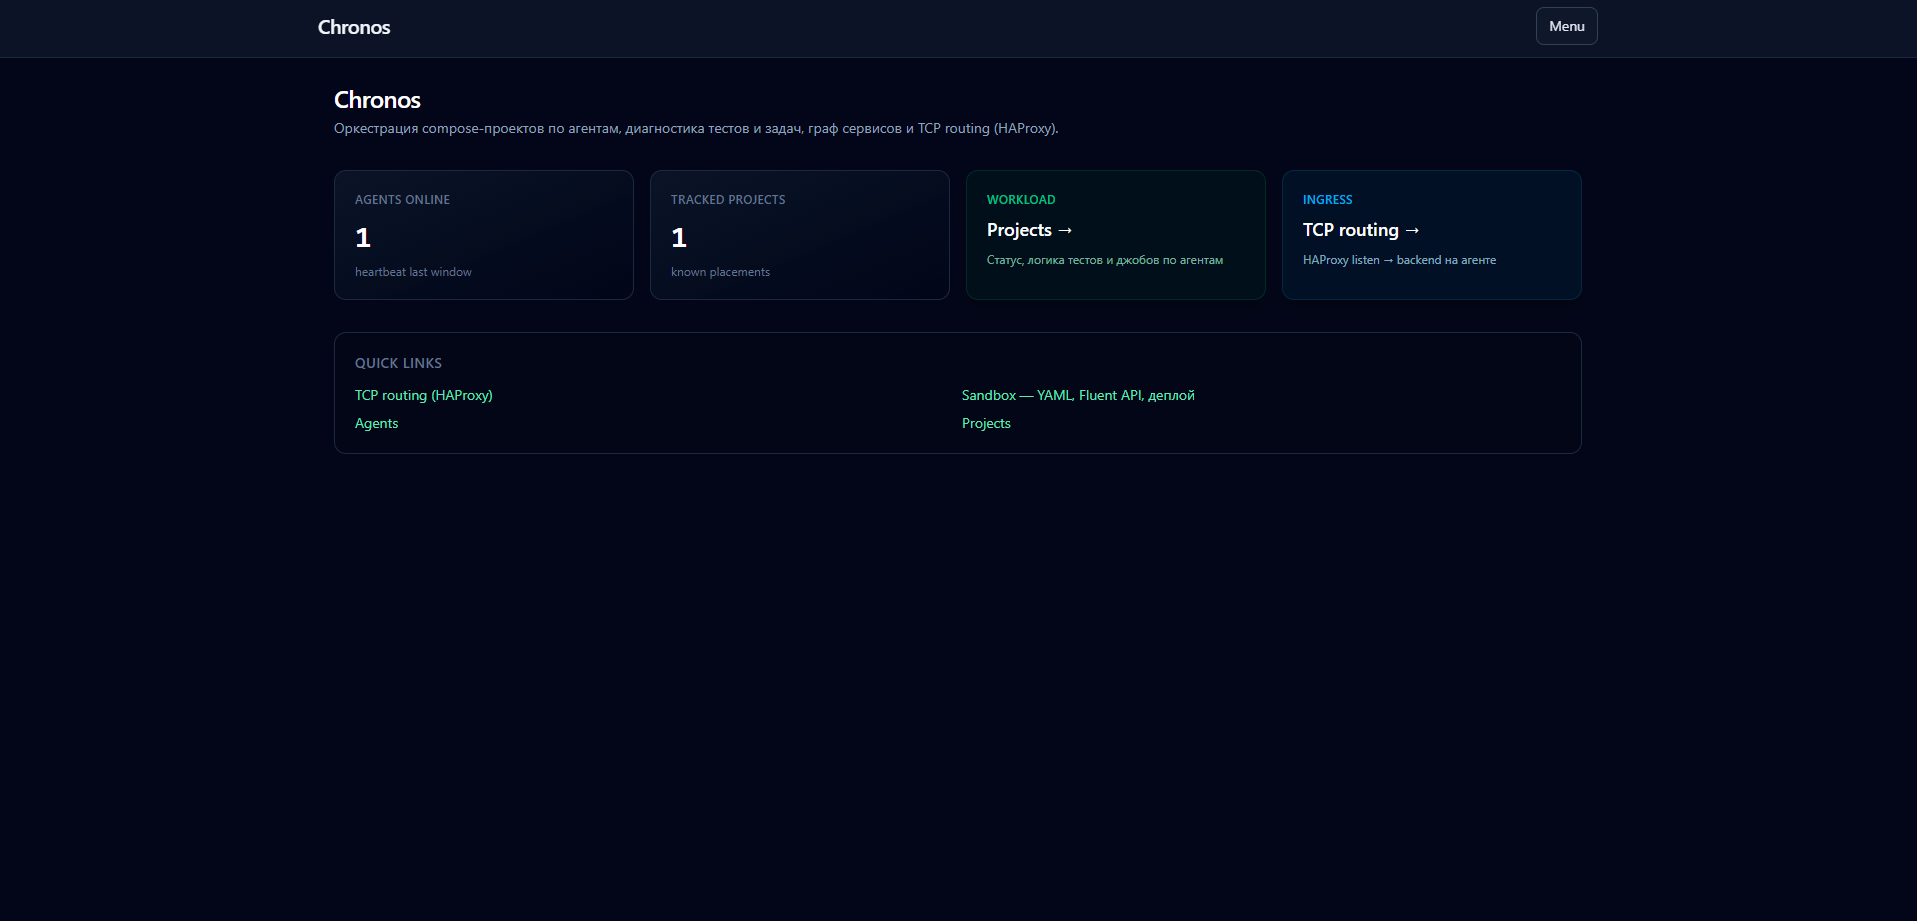
\includegraphics[width=0.94\linewidth]{ui.dashboard/1.png}%
  }{%
    \IfFileExists{фото/ui.dashboard/1.jpg}{%
      
\includegraphics[width=0.94\linewidth]{ui.dashboard/1.jpg}%
    }{%
      \begin{minipage}{0.94\linewidth}\centering
        \fcolorbox{black}{gray!8}{%
          \begin{minipage}{0.92\linewidth}\centering
            \vspace{1.2cm}
            {\small\textit{Скриншот дашборда (\texttt{/ui/dashboard}): положите кадр в \texttt{фото/ui.dashboard/1.png} или \texttt{1.jpg}.}}
            \vspace{1.2cm}
          \end{minipage}}
      \end{minipage}%
    }%
  }
  \caption{Главная панель (дашборд) веб-интерфейса}
  \label{fig:ui-dashboard}
\end{figure}

\begin{figure}[!ht]
  \centering
  \IfFileExists{фото/ui.agents/1.jpg}{%
    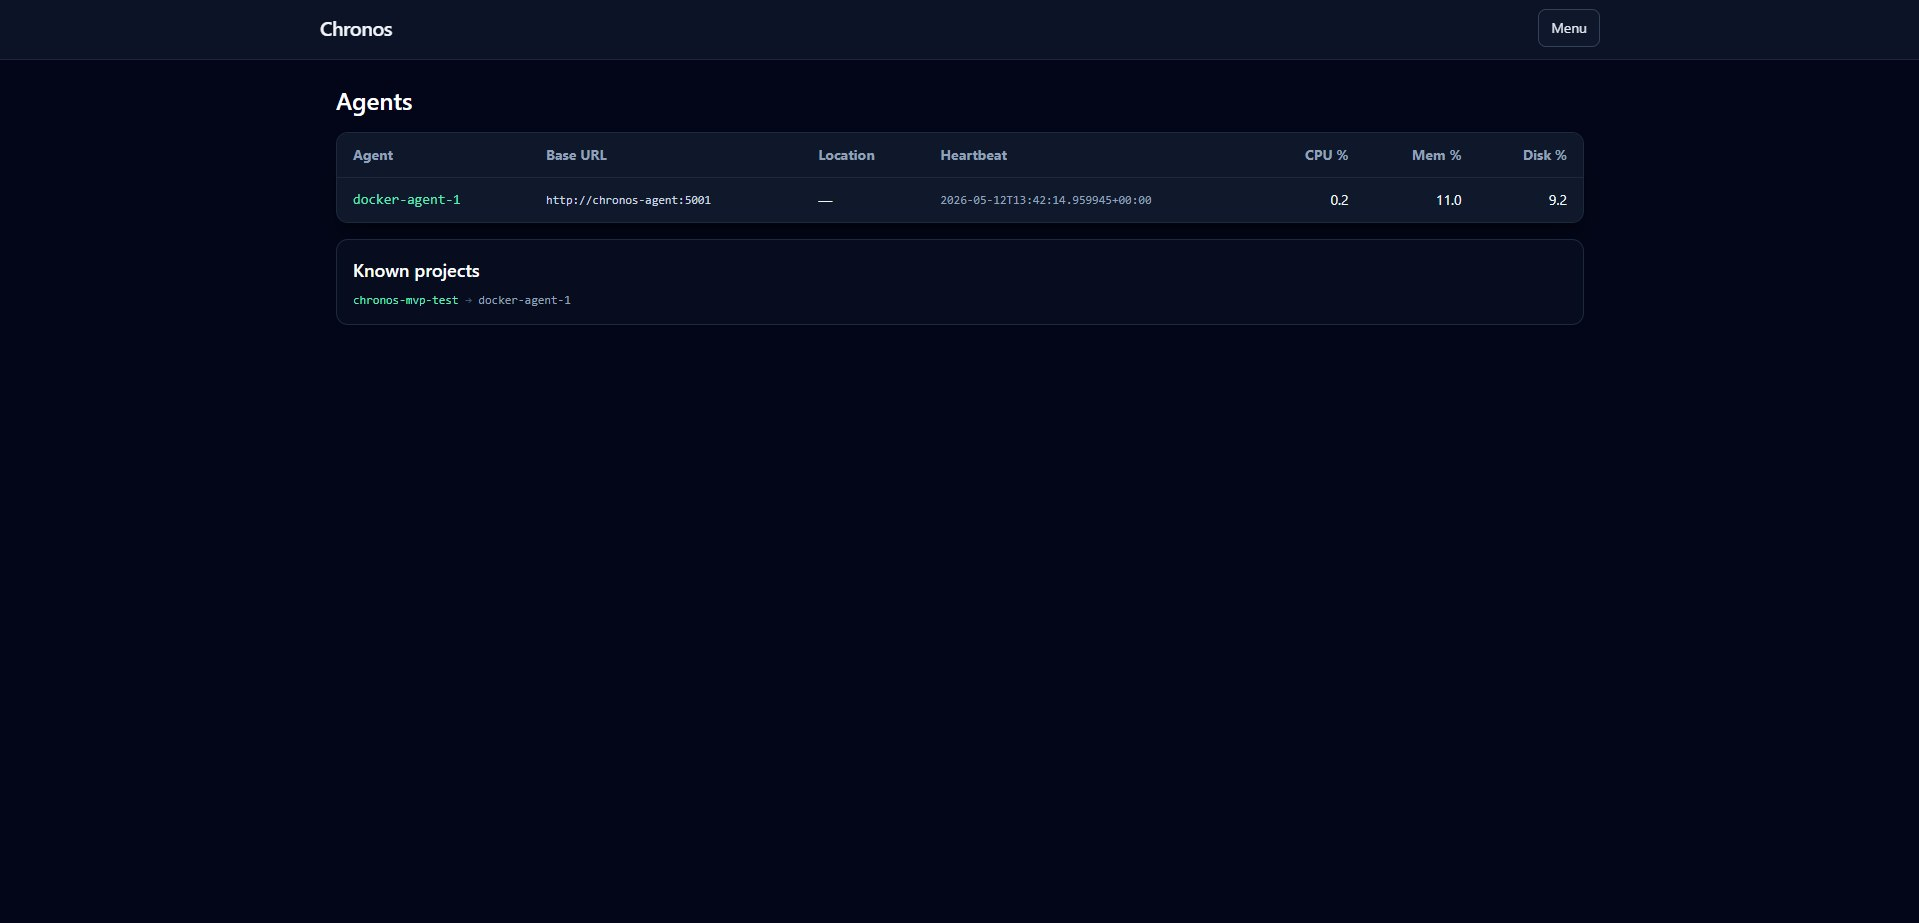
\includegraphics[width=0.94\linewidth]{ui.agents/1.jpg}%
  }{%
    \begin{minipage}{0.94\linewidth}\centering
      \fcolorbox{black}{gray!8}{%
        \begin{minipage}{0.92\linewidth}\centering
          \vspace{1.2cm}
          {\small\textit{Скриншот списка агентов (\texttt{/ui/agents}): положите кадр в \texttt{фото/ui.agents/1.jpg}.}}
          \vspace{1.2cm}
        \end{minipage}}
    \end{minipage}%
  }
  \caption{Список агентных узлов}
  \label{fig:ui-agents}
\end{figure}

\begin{figure}[!ht]
  \centering
  \IfFileExists{фото/ui.projects.list/1.jpg}{%
    
\includegraphics[width=0.94\linewidth]{ui.projects.list/1.jpg}%
  }{%
    \begin{minipage}{0.94\linewidth}\centering
      \fcolorbox{black}{gray!8}{%
        \begin{minipage}{0.92\linewidth}\centering
          \vspace{1.2cm}
          {\small\textit{Положите скриншот списка проектов в файл \texttt{фото/ui.projects.list/1.jpg} (отдельно от кадров карточки проекта в \texttt{ui.projects/}).}}
          \vspace{1.2cm}
        \end{minipage}}
    \end{minipage}%
  }
  \caption{Список compose-проектов кластера}
  \label{fig:ui-projects}
\end{figure}

\begin{figure}[!ht]
  \centering
  
\includegraphics[width=0.94\linewidth]{ui.projects/1.jpg}\\[2mm]
  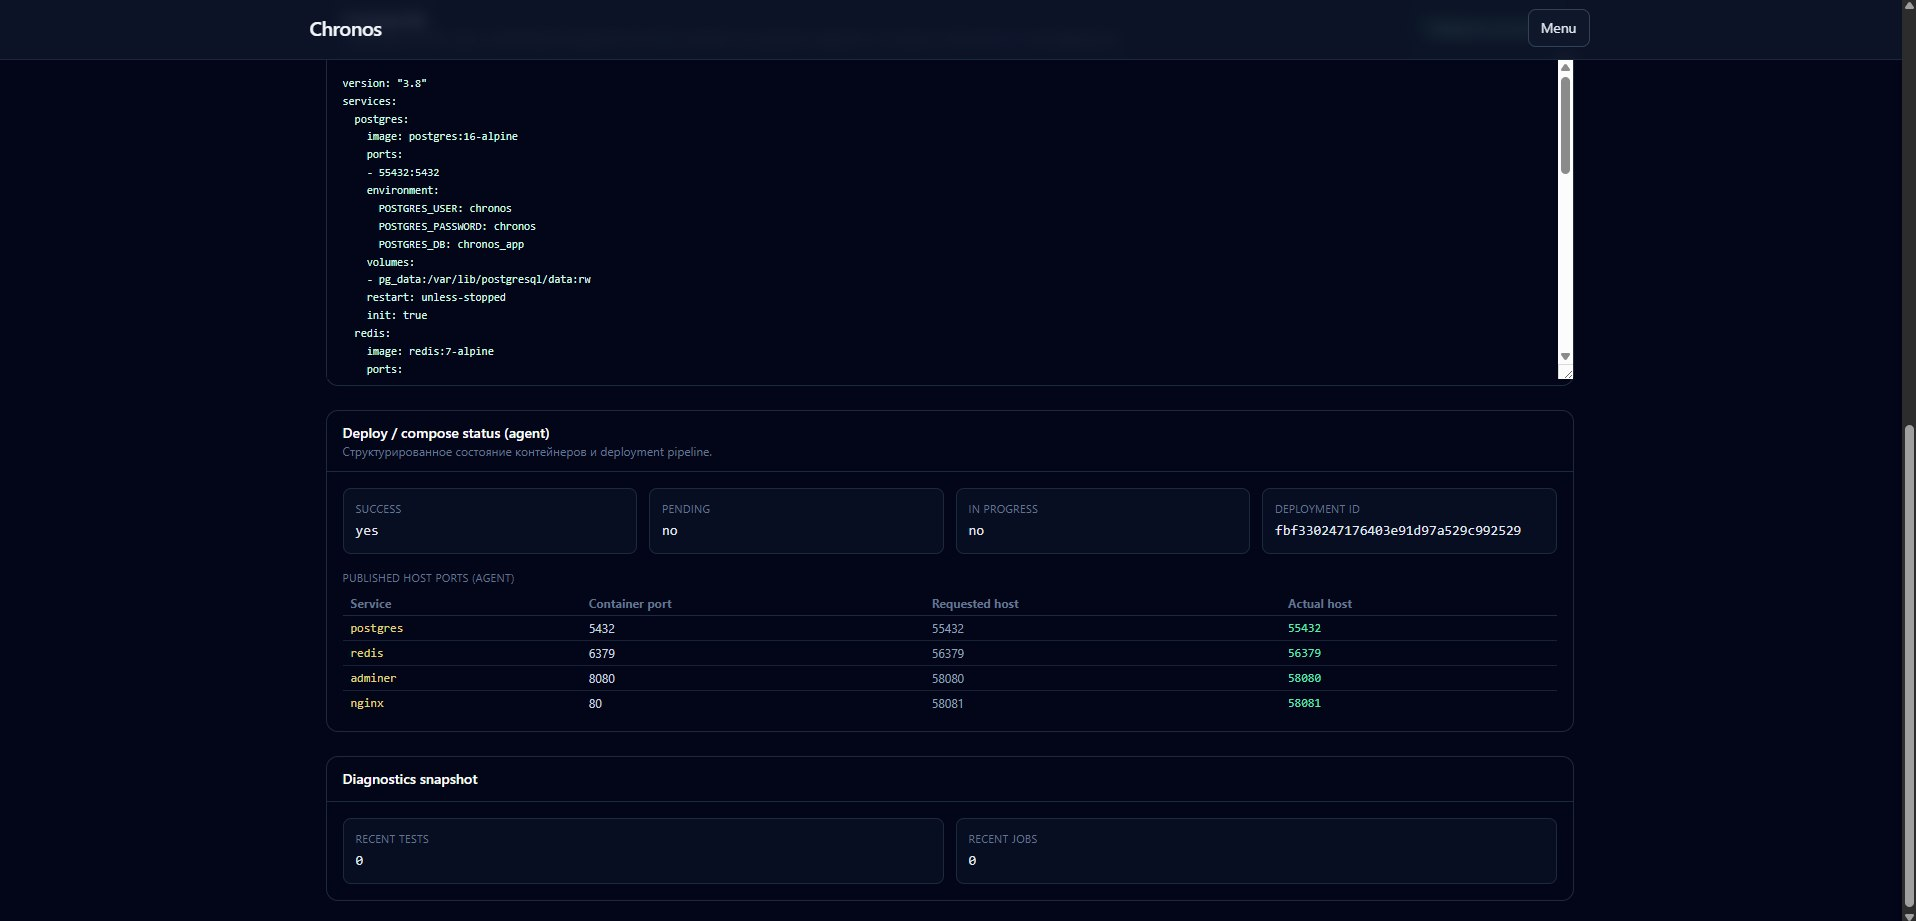
\includegraphics[width=0.94\linewidth]{ui.projects/2.jpg}
  \caption{Детальная страница проекта}
  \label{fig:ui-project-detail}
\end{figure}

\begin{figure}[!ht]
  \centering
  
\includegraphics[width=0.94\linewidth]{ui.projects.archive/1.jpg}
  \caption{Архивированные проекты}
  \label{fig:ui-archived}
\end{figure}

\begin{figure}[!ht]
  \centering
  
\includegraphics[width=0.94\linewidth]{ui.routing/1.jpg}\\[2mm]
  
\includegraphics[width=0.94\linewidth]{ui.routing/2.jpg}
  \caption{Управление TCP-маршрутизацией (HAProxy)}
  \label{fig:ui-routing}
\end{figure}

\begin{figure}[!ht]
  \centering
  
\includegraphics[width=0.94\linewidth]{ui.sandbox/1.jpg}\\[2mm]
  
\includegraphics[width=0.94\linewidth]{ui.sandbox/2.jpg}\\[2mm]
  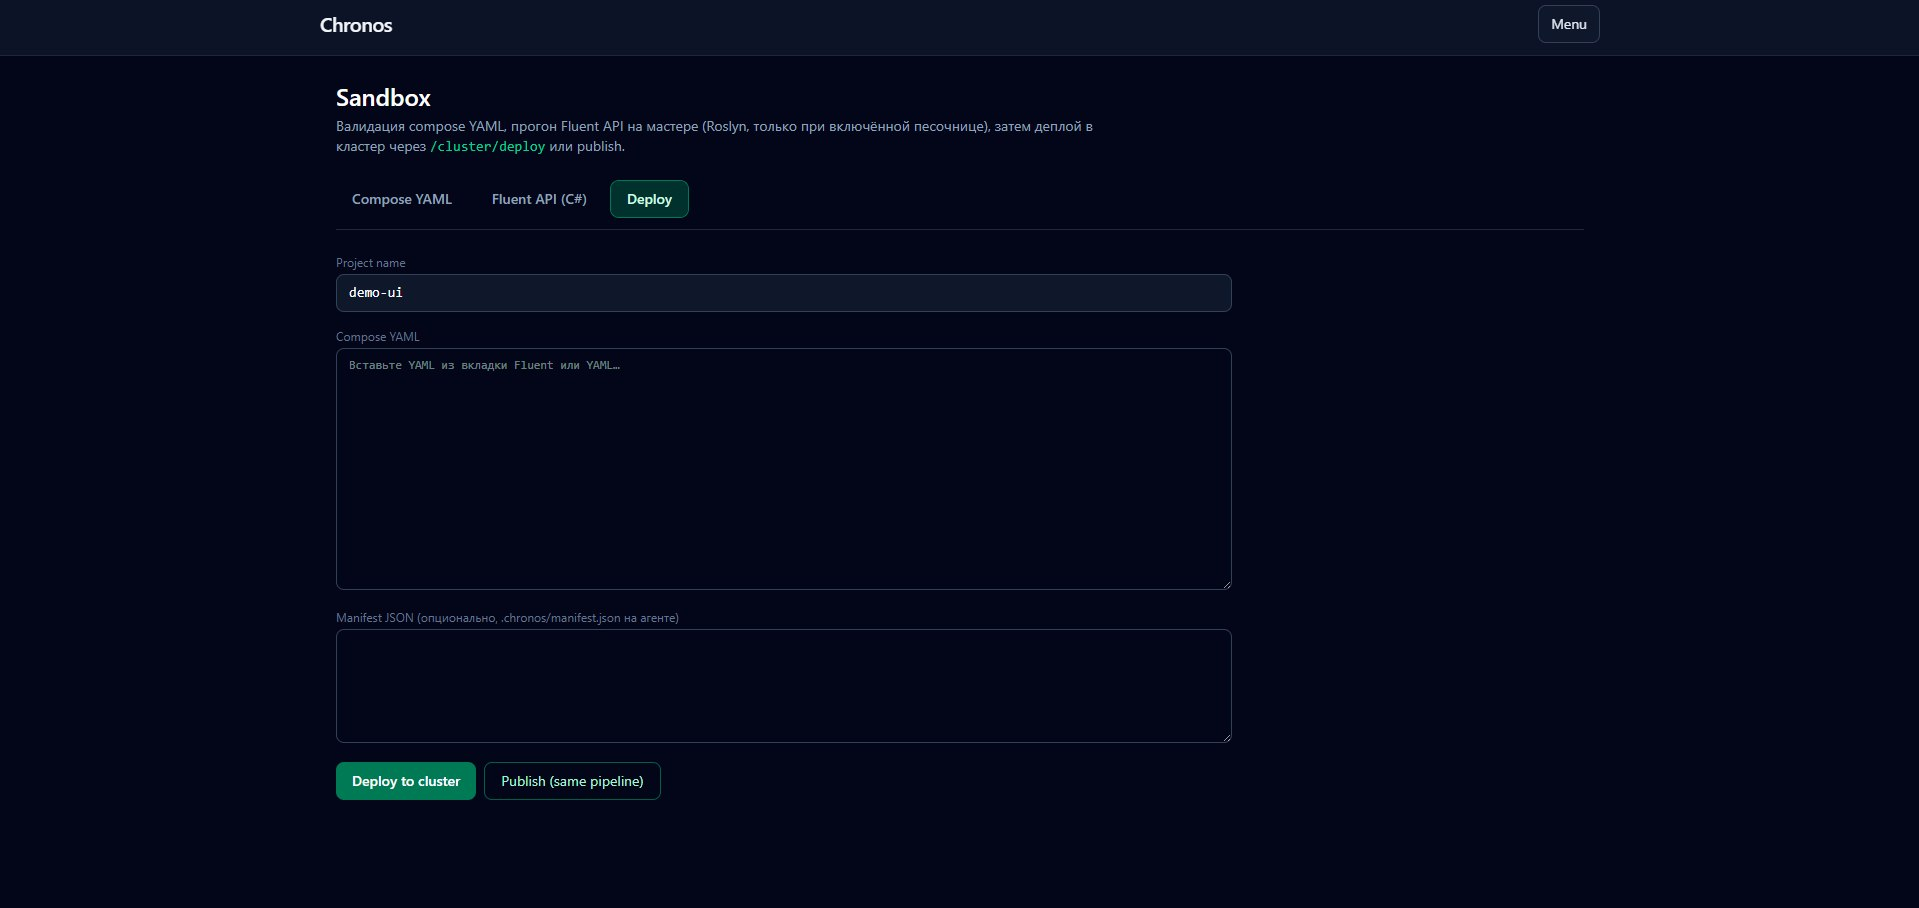
\includegraphics[width=0.94\linewidth]{ui.sandbox/3.jpg}
  \caption{Песочница YAML и Fluent API}
  \label{fig:ui-sandbox}
\end{figure}


\subsection{Практическая часть: запуск из кода}

Практическая демонстрация возможностей Chronos.Core заключается в программном создании экземпляра \texttt{ComposeBuilder}, описании сервисов, портов и томов, вызове валидации и методов \texttt{PublishRemoteAsync}/\texttt{StartRemoteAsync} (или локального \texttt{StartAsync}) с указанием URL агента и ключа API.

\textit{В данной версии текста ВКР листинги конкретного кода автора (фрагменты из репозитория или учебного примера) вставляются в этот подраздел вручную по согласованию с научным руководителем, чтобы сохранить актуальность строк и номеров файлов.} Рекомендуется включить:
\begin{itemize}[leftmargin=1.5cm]
  \item минимальный пример построения одного сервиса с публикацией порта;
  \item пример добавления артефакта деплоя;
  \item пример вызова удалённого старта после \texttt{PublishAsync}.
\end{itemize}

\subsection{Безопасность}

Реализованы проверки API-ключей, ограничения на опасные команды, редактирование потенциально чувствительных подстрок в логах. Для production-развёртывания рекомендуется дополнительно вынести секреты в внешние хранилища и ограничить сетевой доступ к \texttt{docker.sock} на хосте агента.

\section{Экспериментальная проверка и оценка результатов}

\subsection{Методика испытаний}

Проверка системы проводилась на локальном стенде, поднимаемом из \texttt{deploy/docker/docker-compose.yml}. Перед началом серии тестов фиксировались версии образов (Master, Agent, PostgreSQL, HAProxy, Loki, Grafana) и параметры переменных окружения, влияющих на диапазон TCP-портов и пути динамической конфигурации HAProxy.

\textbf{Сценарии.} Набор проверок согласован с каталогом функциональных сценариев в приложении~Б: регистрация и heartbeat агента, публикация и жизненный цикл compose-проекта, добавление и удаление TCP-маршрутов (в том числе с автоматическим listen), перезагрузка HAProxy после изменения файла, отказ при конфликте порта, просмотр сгенерированного конфига в UI. Для каждого сценария фиксировались: входные данные, ожидаемый результат по критериям ниже, фактический статус HTTP и наблюдения в логах Loki.

\textbf{Контроль среды.} Отдельно проверялась согласованность сетевой модели Docker: доступность \texttt{host.docker.internal} из контейнера HAProxy к порту, опубликованному compose на хосте агента. На Linux-хостах без Docker Desktop эквивалентная схема может потребовать иной адресации backend --- это зафиксировано как ограничение стенда, а не как дефект кода при условии корректной настройки.

\textbf{Воспроизводимость.} Каждый ключевой сценарий выполнялся минимум дважды: «холодный'' старт после \texttt{docker compose up} и «тёплый'' повтор с уже заполненной БД и существующими маршрутами. Это выявляет ошибки инициализации и ошибки, связанные с накопленным состоянием.

\subsection{Критерии успешности}

Сценарий считается успешным, если выполняются условия:
\begin{itemize}[leftmargin=1.5cm]
  \item API возвращает консистентный статус и понятные диагностические сообщения;
  \item в UI отображается фактическое состояние маршрутов;
  \item сгенерированный \texttt{chronos-tcp.cfg} проходит валидацию HAProxy;
  \item TCP-подключения по listen-порту доходят до целевого backend-порта;
  \item перезапуск компонентов не приводит к потере критического состояния.
\end{itemize}

\subsection{Результаты функциональных испытаний}

В результате испытаний подтверждено:
\begin{itemize}[leftmargin=1.5cm]
  \item корректное добавление маршрутов с автоматическим выбором listen-порта в допустимом диапазоне;
  \item корректное удаление маршрутов и обновление конфигурации прокси;
  \item стабильная работа сценария проксирования к \texttt{host.docker.internal:PORT};
  \item успешное отображение маршрутов и их состояния в UI.
\end{itemize}

\textbf{Соответствие каталогу сценариев.} Сценарии F-01--F-04 (регистрация, heartbeat, публикация, запуск) и F-07--F-14 (TCP-маршруты, reload HAProxy, доступ к backend, просмотр cfg) на стенде автора выполнены успешно. Сценарии F-15--F-18 (песочница, очистка агентов, аудит, повторный подъём) проверялись выборочно: подтверждена работоспособность путей, критичных для демонстрации дипломного прототипа; полный регрессионный прогон рекомендуется вынести в отдельный контур CI.

Выявленные и устраненные в процессе реализации дефекты:
\begin{itemize}[leftmargin=1.5cm]
  \item ошибка HAProxy при наличии UTF-8 BOM в начале динамического конфига;
  \item проблемы запуска shell-скрипта перезагрузки при CRLF-окончаниях строк;
  \item неоднозначность пользовательской интерпретации backend-портов (порт контейнера vs порт хоста).
\end{itemize}

\subsection{Ограничения эксперимента}

Испытания носят функциональный характер: не измерялись предельная пропускная способность TCP-прокси, задержки при одновременной публикации десятков проектов и деградация БД при длительном накоплении аудита. Нагрузочное тестирование и формализованный отчёт SLA не входили в объём работы и относятся к направлениям развития.

\subsection{Обсуждение результатов}

Полученные результаты подтверждают рабочую гипотезу: для существенной доли практических задач возможно построить инженерно пригодную оркестрацию на основе Compose без перехода на тяжелые кластерные платформы. Ключевым фактором является наличие централизующего слоя (Master + UI) и стандартизованного агентного контура.

Система показала устойчивость в условиях частых изменений маршрутов и конфигураций. Наиболее критичные риски концентрируются в эксплуатационной плоскости:
\begin{itemize}[leftmargin=1.5cm]
  \item ошибки в сетевой адресации backend;
  \item неконсистентность окружения (различия Docker Desktop и Linux host-mode);
  \item неверная трактовка опубликованных портов.
\end{itemize}

\subsection{Направления дальнейшего развития}

В рамках следующих итераций целесообразно реализовать:
\begin{enumerate}[leftmargin=1.5cm]
  \item multi-master режим с отказоустойчивым лидерством;
  \item расширенную модель авторизации и ролей;
  \item автоматический discovery опубликованных портов compose-проектов агента;
  \item формализованные нагрузочные бенчмарки и тесты деградации;
  \item расширенную интеграцию с внешними системами наблюдаемости.
\end{enumerate}

\section{Заключение}

В работе спроектирован и реализован программный комплекс \textbf{Chronos} --- платформа для централизованного управления Docker Compose-проектами на нескольких узлах с веб-интерфейсом, динамической TCP-маршрутизацией через HAProxy, политиками резервного копирования томов в объектное хранилище и централизованным сбором логов в связке Loki/Grafana.

Достигнуты следующие результаты:
\begin{itemize}[leftmargin=1.5cm]
  \item обоснована актуальность подхода «compose + управляющий контур'' на фоне Kubernetes и классических панелей управления Docker;
  \item сформулированы и реализованы требования к модульной архитектуре (Core, Agent, Master, Web);
  \item реализованы публикация проектов, удалённое управление жизненным циклом, регистрация агентов, декларативные проверки и артефакты деплоя;
  \item внедрены механизмы снимков томов, фоновой репликации по политикам Master и интеграции с S3-совместимым API;
  \item реализован реестр TCP-маршрутов с генерацией конфигурации HAProxy и сценарием динамического применения на стенде;
  \item подтверждена работоспособность решения на локальном docker-compose стенде.
\end{itemize}

Практический итог --- работающий комплекс, который \textbf{уже применяется автором локально} для управления собственной инфраструктурой разработки: развёртывание сервисов, маршрутизация портов и наблюдаемость сведены к единому контуру без обязательного перехода на Kubernetes.

Направления развития включают усиление отказоустойчивости Master, расширение модели доступа, автоматизацию подсказок по портам из состояния compose и расширенные нагрузочные испытания.

\textbf{Цель работы достигнута}, поставленные задачи решены.


\clearpage
\printbibliography[title={Список использованных источников}]

\appendix
\section{Приложение А. Фрагменты конфигураций}

\subsection{Фрагмент docker-compose стенда}

\begin{lstlisting}[style=code,language={},caption={Ключевые части deploy/docker/docker-compose.yml}]
services:
  haproxy:
    image: haproxy:3.0-alpine
    entrypoint: ["/bin/sh", "/usr/local/etc/haproxy/run-with-dynamic-reload.sh"]
    extra_hosts:
      - "host.docker.internal:host-gateway"
    ports:
      - "18404:8404"
      - "5002-5099:5002-5099"

  chronos-master:
    environment:
      CHRONOS_HAPROXY_DYNAMIC_DIR: /haproxy-dynamic
      CHRONOS_HAPROXY_LISTEN_PORT_MIN: "5002"
      CHRONOS_HAPROXY_LISTEN_PORT_MAX: "5099"
      CHRONOS_HAPROXY_TCP_SUGGESTED_BACKEND_HOST: host.docker.internal
\end{lstlisting}

\subsection{Фрагмент алгоритма выбора listen-порта}

\begin{lstlisting}[style=code,language=C,caption={Логика выделения listen-порта}]
internal static int? Allocate(int preferred, HashSet<int> reservedByRoutes,
    int maxScan, int? listenMin, int? listenMax)
{
    // 1) нормализация диапазона
    // 2) перебор candidate = preferred + i
    // 3) пропуск занятых или невалидных портов
    // 4) возврат первого подходящего порта
}
\end{lstlisting}

\section{Приложение Б. Каталог сценариев и эксплуатационные материалы}

\subsection{Каталог функциональных сценариев}

\begin{longtable}{p{0.08\textwidth}p{0.28\textwidth}p{0.56\textwidth}}
\toprule
ID & Сценарий & Критерий приемки \\
\midrule
\endfirsthead
\toprule
ID & Сценарий & Критерий приемки \\
\midrule
\endhead
F-01 & Регистрация агента & После старта Agent появляется в списке Master с валидным \texttt{agentId} и \texttt{baseUrl}. \\
F-02 & Heartbeat агента & Поле последнего heartbeat обновляется периодически, агент не удаляется TTL-процедурой. \\
F-03 & Публикация compose-проекта & API возвращает успешный статус, на диске агента сохраняется compose-файл проекта. \\
F-04 & Запуск проекта & После команды start сервисы переходят в состояние running, статус доступен через API. \\
F-05 & Остановка проекта & После stop сервисы удаляются/останавливаются в соответствии с настройками. \\
F-06 & Чтение логов & Запрос логов возвращает поток строк по выбранному сервису без критических ошибок. \\
F-07 & Добавление TCP-маршрута (auto) & При пустом listen выбирается первый доступный порт в диапазоне master-конфига. \\
F-08 & Добавление TCP-маршрута (fixed) & При явном listen в допустимом диапазоне маршрут сохраняется и отображается в UI. \\
F-09 & Отказ при конфликте listen-порта & API возвращает информативную ошибку, состояние реестра не изменяется. \\
F-10 & Удаление TCP-маршрута & Маршрут удаляется из JSON и cfg, в UI больше не отображается. \\
F-11 & Релоад HAProxy после изменения cfg & Изменение файла приводит к HUP-сигналу и применению новых listen без ручного вмешательства. \\
F-12 & Проверка BOM-защиты & При обнаружении BOM в cfg конфигурация переписывается в UTF-8 без BOM. \\
F-13 & Доступ к backend на хосте & Маршрут \texttt{host.docker.internal:PORT} проходит health check и пропускает TCP-трафик. \\
F-14 & Просмотр сгенерированного cfg в UI & Пользователь видит актуальный текст динамического конфига для диагностики. \\
F-15 & Sandbox Fluent preview & Код в sandbox формирует YAML или возвращает контролируемую ошибку валидации. \\
F-16 & Очистка stale agents & Фоновая задача удаляет неактивных агентов по заданному TTL. \\
F-17 & Аудит операций & Критичные действия фиксируются в журнале аудита в базе Master. \\
F-18 & Повторный подъем стека & После рестарта compose состояние маршрутов и БД консистентно восстанавливается. \\
\bottomrule
\end{longtable}

\subsection{Набор эксплуатационных рисков и мер снижения}

\begin{longtable}{p{0.3\textwidth}p{0.28\textwidth}p{0.34\textwidth}}
\toprule
Риск & Вероятное проявление & Мера снижения \\
\midrule
\endfirsthead
\toprule
Риск & Вероятное проявление & Мера снижения \\
\midrule
\endhead
Несоответствие backend host топологии & TCP health check в HAProxy в состоянии DOWN & Использование \texttt{host.docker.internal} для хостовых портов, явная документация в UI. \\
Конфликт listen-портов & Отказ добавления маршрута или bind error при старте HAProxy & Диапазон listen в env, проверка занятости и резервирования портов в реестре. \\
CRLF в shell-скриптах & Ошибки \texttt{illegal option} при запуске entrypoint & Правило \texttt{.gitattributes} и контроль формата файлов в CI. \\
BOM в динамическом cfg & Ошибка парсинга HAProxy \texttt{unknown keyword} на первой строке & Принудительная запись UTF-8 without BOM и автоисправление при загрузке. \\
Некорректный HUP/reload & Маршрут добавлен в файл, но не применен процессом & Автоматический watcher-скрипт и явные health checks. \\
Проблемы доступности БД & Ошибки при старте Master/Agent или миграциях & Health checks postgres, отложенный запуск сервисов по \texttt{depends\_on}. \\
Рост аудита без контроля retention & Деградация БД по размеру таблиц & Периодическая очистка старых записей по configurable retention. \\
Неоднозначность user input в UI & Пользователь указывает контейнерный порт вместо хостового и наоборот & Контекстные подсказки и информативные ошибки API. \\
\bottomrule
\end{longtable}

\subsection{Расширенный шаблон экспериментальной главы}

Ниже приведен текстовый шаблон, который может быть использован для расширения основной главы результатов до полного стандарта кафедральной ВКР. Каждый подраздел рекомендуется дополнять таблицами замеров, скриншотами и логами запусков.

\textbf{1. Описание аппаратно-программного стенда.}
Указать характеристики хоста (CPU, RAM, диск), версию операционной системы, версии Docker Engine, Docker Compose, .NET SDK/runtime, браузера для UI-тестов и сетевые ограничения. Важно фиксировать точные версии образов (\texttt{postgres:16-alpine}, \texttt{haproxy:3.0-alpine}, \texttt{grafana/grafana:11.3.0}, \texttt{grafana/loki:3.1.1}), поскольку различия в минорных релизах влияют на воспроизводимость.

\textbf{2. Методика проведения измерений.}
Определить повторяемые процедуры: число прогонов каждого сценария, метод фиксации времени (например, timestamp логов), критерии успешности и правила отброса выбросов. Для корректного сравнения важно разделять ``холодный'' запуск (первый старт после поднятия образов) и ``теплый'' запуск (повторный запуск без пересборки).

\textbf{3. Серия экспериментов по маршрутизации.}
Эксперименты рекомендуется разделить на: а) добавление 1 маршрута; б) добавление серии маршрутов; в) удаление и повторное добавление; г) сценарий конфликтующих listen-портов; д) сценарий недоступного backend. Для каждого эксперимента фиксировать: время отклика API, время применения конфигурации HAProxy, фактическую доступность конечного backend.

\textbf{4. Эксперименты устойчивости.}
Проверить поведение при рестарте контейнера HAProxy, Master и Agent, а также при рестарте всего compose-стека. Ключевая проверка: после восстановления маршруты должны остаться консистентными в JSON-реестре, UI и runtime-состоянии HAProxy.

\textbf{5. Эксперименты ошибок ввода.}
Проверить реакции на пустой backend host, нечисловой backend port, порт вне диапазона 1--65535, listen-порт вне опубликованного диапазона, дублирование listen-порта. Для диплома важно показать не только ``happy path'', но и инженерную зрелость обработки ошибок.

\textbf{6. Анализ результатов.}
Сформулировать выводы: какие сценарии устойчивы, где система требует операторской квалификации, какие ошибки перехватываются автоматически, а какие остаются зоной ответственности инженера эксплуатации.

\subsection{Таблица API-эндпоинтов для документирования}

{\small\raggedright
\begin{longtable}{
  >{\raggedright\arraybackslash}p{0.26\textwidth}
  >{\raggedright\arraybackslash}p{0.12\textwidth}
  >{\raggedright\arraybackslash}p{0.18\textwidth}
  >{\raggedright\arraybackslash}p{0.38\textwidth}}
\toprule
Путь & Метод & Подсистема & Назначение \\
\midrule
\endfirsthead
\toprule
Путь & Метод & Подсистема & Назначение \\
\midrule
\endhead
\path{/agents/register} & POST & Master API & Регистрация агентного узла в реестре Master. \\
\path{/agents/{id}/heartbeat} & POST & Master API & Обновление heartbeat агента и метрик состояния. \\
\path{/agents} & GET & Master API & Получение списка активных и исторических агентных узлов. \\
\path{/api/v1/haproxy/tcp-routes} & GET & UI API & Чтение списка маршрутов и сгенерированного HAProxy cfg. \\
\path{/api/v1/haproxy/tcp-routes} & POST & UI API & Добавление TCP-маршрута с валидацией listen/backend параметров. \\
\path{/api/v1/haproxy/tcp-routes/{id}} & DELETE & UI API & Удаление маршрута по идентификатору. \\
\path{/api/v1/sandbox/fluent-preview} & POST & UI API & Выполнение sandbox-просмотра Fluent-кода и генерация YAML. \\
\path{/projects} & GET & Agent API & Список compose-проектов на агентном узле. \\
\path{/projects/{name}/status} & GET & Agent API & Статус конкретного проекта и контейнеров. \\
\path{/projects/{name}/logs} & GET & Agent API & Логи сервисов compose-проекта. \\
\bottomrule
\end{longtable}
}


\end{document}
